%% 
%% Copyright 2019-2024 Elsevier Ltd
%% 
%% Version 2.4
%% 
%% This file is part of the 'CAS Bundle'.
%% --------------------------------------
%% 
%% It may be distributed under the conditions of the LaTeX Project Public
%% License, either version 1.2 of this license or (at your option) any
%% later version.  The latest version of this license is in
%%    http://www.latex-project.org/lppl.txt
%% and version 1.2 or later is part of all distributions of LaTeX
%% version 1999/12/01 or later.
%% 
%% The list of all files belonging to the 'CAS Bundle' is
%% given in the file `manifest.txt'.
%% 
%% Template article for cas-sc documentclass for 
%% single column output.

%\documentclass[a4paper,fleqn,longmktitle]{cas-sc}
\documentclass[a4paper]{cas-sc}

\usepackage[numbers]{natbib}
%\usepackage[authoryear]{natbib}
%\usepackage[authoryear,longnamesfirst]{natbib}

%%%Author macros
\def\tsc#1{\csdef{#1}{\textsc{\lowercase{#1}}\xspace}}
\tsc{WGM}
\tsc{QE}
\tsc{EP}
\tsc{PMS}
\tsc{BEC}
\tsc{DE}
%%%
\usepackage{amssymb,amsmath}
\usepackage{url}
\usepackage{xcolor}
\usepackage{bm}
\usepackage{placeins}
\usepackage{hyperref}
\usepackage{longtable} % en el preámbulo
\usepackage[capitalise]{cleveref}
\usepackage{graphicx}
\DeclareGraphicsExtensions{.pdf,.png,.jpg,.jpeg}
\usepackage{pifont}% http://ctan.org/pkg/pifont
\newcommand{\cmark}{\ding{51}}%
\newcommand{\xmark}{\ding{55}}%

\usepackage{array}
\newcolumntype{C}[1]{>{\centering\let\newline\\\arraybackslash\hspace{0pt}}m{#1}}

%%Defining some useful variables 
\providecommand{\ve}[1]{{\bm{#1}}}%
\providecommand{\mat}[1]{{\bm{#1}}} %
\providecommand{\var}[1]


\DeclareMathOperator{\subconj}{\negthinspace\subset\negthinspace }
\DeclareMathOperator{\en}{\!\,\in\!\,}
\DeclareMathOperator{\igual}{\!\,=\!\,}
\DeclareMathOperator{\dist}{\operatorname{d}}
\DeclareMathOperator{\xx}{\negthickspace\times\negthickspace}
\providecommand{\s}[1]{\negthinspace#1\negthinspace}%

\begin{document}

\newcommand{\Real}{\mathbb{R}}
\newcommand{\N}{\mathbb{N}}
\newcommand{\Z}{\mathbb{Z}}
\newcommand{\X}{\mathcal{X}}
\newcommand{\Y}{\mathcal{Y}}
\newcommand{\boldV}{\mathbf{V}}
\newcommand{\dataset}{{\cal D}}
\newcommand{\gauss}{\mathcal{N}} 

\providecommand{\ch}[1]{\textcolor{blue!50}{#1}}

\let\WriteBookmarks\relax
\def\floatpagepagefraction{1}
\def\textpagefraction{.001}
\shorttitle{}
\shortauthors{J. Méndez-Rondón et~al.}
%\begin{frontmatter}

\title [mode = title]{\textcolor{blue}{Regression‑based Explainable Deep Learning for Estimating Magnetic Hamiltonian Parameters from Nanodots Domain Images}}
%An Explainable Deep Learning Approach for Image-based Prediction of Magnetic Parameters in Nanodots
%\tnotemark[1]

\author[1]{J. {Méndez-Rondón}}[]
\cormark[1]
\ead{jumendezro@unal.edu.co}

\affiliation[1]{organization={Signal Processing and Recognition Group, Universidad Nacional de Colombia, Sede Manizales},postcode={170001}}

\author[1]{M. {García-Quimbayo}}[]
\ead{migarciaq@unal.edu.co}

\author[2]{J. {Agudelo-Giraldo}}[]
\ead{josed.agudelog@autonoma.edu.co}

\affiliation[2]{organization={Departamento de Física y Matemáticas,  Universidad Autónoma de Manizales},postcode={170002}}

\author[3]{J. {Montes-Monsalve}}[]
\ead{jimontesm@unal.edu.co}

\author[1]{A. {Álvarez-Meza}}[]
\ead{amalvarezme@unal.edu.co }



\affiliation[3]{organization={Dirección Académica, Universidad Nacional de Colombia, Sede La Paz},postcode={XXX}}





\cortext[cor1]{Corresponding author}
%El estudio de los dominios magnéticos en materiales a nanoescala es fundamental para el desarrollo de tecnologías emergentes en espintrónica, biomedicina y almacenamiento de energía. Sin embargo, la comprensión cuantitativa de estos dominios a partir de imágenes experimentales sigue siendo limitada debido a la complejidad que implica inferir los parámetros físicos  subyacentes. Esta desconexión entre la visualización experimental y los modelos físicos dificulta tanto la validación teórica como la predicción del comportamiento magnético en nuevos materiales funcionales. Los modelos de aprendizaje profundo pueden contribuir significativamente al análisis de sistemas complejos, permitiendo la extracción de patrones, la predicción de propiedades y el establecimiento de relaciones entre los datos experimentales y variables ocultas que serían difíciles de identificar mediante enfoques tradicionales. No obstante, su aplicación en tareas de estimación de parámetros físicos enfrenta grandes desafíos, como la existencia de múltiples soluciones posibles que pueden dar lugar a patrones visuales similares, lo que dificulta la identificación de un conjunto único de parámetros compatibles con una observación dada, así como la limitada interpretabilidad de las redes neuronales profundas, que impide saber con certeza si las predicciones se basan en principios físicos reales o en correlaciones estadísticas débilmente generalizables. En este trabajo, proponemos un método basado en redes convolucionales para estimar parámetros físicos a partir de dominios magnéticos, que permite no solo la predicción, sino también la interpretación del espacio latente de la red, facilitando así una mejor comprensión de las relaciones físicas subyacentes.

\begin{abstract}
%%%%%%%%%%%%%%%%%%%%%%%%%%%%%%%%%%%%%%%%%%%%%%%%%%%%%%%%%%%%%%%%%%
%%%% EXPLICACIÓN DE NANODISCOS Y COMO SE GENERAN LAS IMAGENES. TRANSICIÓN --MARIA --CHECK
%%%%%
%%%%%%%%%%%%%%%%%%%%%%%%%%
%%%% CONCLUSIÓN  --JUAN --CHECK
%%%%%%%%%%%%%%%%%%%%%%%%%%%%%%%%%%%%%%
%%% EXPLICAR PORQUE NO TRANSFORMERS. --JUAN. YA REVISAMOS
%%%%%%%%%%%%%%%%%%%%%%%%%%%%%%%%%%%%%%
%%%% PROPUESTA ESPECIFICANDO INTERPRETABILIDAD. -- R2. --CHECK
%% PRUEBAS CON CADA TIPO DE HAMILTONEANO ESPECIFICANDO LA BASE DE LOS EXPERIMENTO. --MARIA
%%%% REVISAR NANOPARTICULAS PARA REEMPLAZAR POR NANODOTS. -- REEMPLAZAR TODO POR NANODOTS DESDE PROBLEM STATEMENT. --CHECK
%%% 
%% REEMPLAZAR POR ESTUDIOS A NANO ESCALA. -- MARIA.
%% DESDE EL ABSTRACT COLOCAR LA NOVEDAD EN LA REGRESIÓN A COMPARACIÓN EN MODELOS SIMILARES LLEVADOS A TAREAS DE CLASIFICACIÓN. -- JUAN.
%%%%%%%%%%%%%%%
The investigation of magnetic domain structures in nanoscale materials is essential for advancing emerging technologies in spintronics, biomedicine, and energy storage. \textcolor{blue}{These magnetic textures arise from high-resolution imaging techniques or from simulations that model atomistic spin interactions at the nanoscale}. However, the quantitative interpretation of these domains from experimental images remains challenging due to the complexity of inferring the physical parameters associated. This disconnect between experimental visualization and physical models hinders both theoretical validation and the prediction of magnetic behavior in new functional materials. Deep learning models can significantly contribute to the analysis of complex systems, enabling the extraction of patterns, the prediction of properties, and the establishment of relationships between experimental data and hidden variables that would be difficult to identify using traditional approaches. However, their application in physical parameter estimation tasks faces major challenges, such as the existence of multiple possible solutions that can lead to similar visual patterns, making it difficult to identify a unique set of parameters compatible with a given observation, \textcolor{blue}{the intrinsic variability and noise present in both simulated and experimental datasets further complicate the parameter estimation task. Small perturbations in temperature, anisotropy, or exchange interactions can lead to visually similar spin textures, increasing the risk of degeneracy and instability in regression-based predictions. To mitigate this issue, several studies have reformulated the problem as a classification task, focusing on identifying representative magnetic states or regimes rather than inferring exact numerical values. This strategy reduces sensitivity to noise, improves robustness against non-unique solutions, and provides a more tractable pathway for analyzing highly complex or disordered configurations where direct parameter estimation becomes unreliable} , as well as the limited interpretability of deep neural networks, which prevents us from knowing with certainty whether predictions are based on real physical principles or on weakly generalizable statistical correlations.\textcolor{blue}{ In this work, we propose a method based on convolutional networks to estimate physical parameters from magnetic domains, allowing not only prediction but also interpretation of the network’s latent space, thus facilitating a better understanding of the underlying physical relationships. As an additional contribution, we introduce a novel interpretability measure for layer-wise activation maps, defined as 
$S(y_{\text{true}}, y_{\text{pred}}) = 1 - |y_{\text{true}} - y_{\text{pred}}|$, 
which highlights the most relevant pixels in the input image by linking prediction accuracy with spatial features. This similarity-based approach provides a physics-informed way to connect model errors with localized image regions, improving transparency and reliability in the analysis of magnetic domain data.} \textcolor{blue}{
     Our results show that DenseNet121 consistently provides the most accurate and generalizable predictions for Hamiltonian parameters, particularly the Dzyaloshinskii–Moriya interaction, while the proposed Regression Activation Maps (RAMs) offer a physics-informed interpretability framework that links prediction reliability with localized magnetic structures. This demonstrates that deep learning models, when combined with tailored explainability strategies, can bridge the gap between experimental magnetic domain images and underlying physical parameters, contributing to more transparent and reliable analyses of complex nanoscale systems.
} 
\end{abstract}



\begin{keywords}
Keyword 1 \sep Keyword 2
\end{keywords}


 \maketitle


\section{Introduction}

%%%%%%%%%%%%%%% MOTIVACION %%%%%%%%%%%%%%%%%%%
% INTRODUCCIÓN AL USO DE DOMINIOS MOTIVACIÓN %
%, the food industry \cite{hua2021recent}, -- QUITAR LA PARTE DE COMIDAS

The understanding of complex physical systems is of broad interest in various fields of engineering \cite{park2021accurate}. In particular, the \textcolor{blue}{nanoscale studies} aimed at the development of electronic devices have impacted medicine \cite{ziental2020titanium} and energy \cite{alkhalayfeh2021overview}, in accordance with the Sustainable Development Goals and the National Development Plan, seeking productivity and competitiveness through science, technology, and innovation \cite{lemos2023plan}.

In this context, \textcolor{blue}{nanoscale studies} have a wide range of applications in various fields due to their unique physical, chemical, and biological properties, particularly standing out in electronics. In this field, they are used in the manufacture of transistors and LEDs, taking advantage of their ability to enhance the performance and efficiency of these devices \cite{khan2022classification}. Materials such as nanocrystalline lead telluride, cadmium sulfide, zinc selenide, and sulfide are fundamental for the production of LEDs in modern displays, where brightness and size are crucial \cite{chouke2022bioinspired}. 

Additionally, \textcolor{blue}{nanoscale studies} facilitate advances in the creation of more efficient and lightweight batteries for portable devices such as mobile phones and laptops, using structures like aerogels that allow greater energy storage with less weight \cite{jeong2022foldable}. In the context of renewable energy and environmental remediation, \textcolor{blue}{nanoscale studies} are used to enhance the efficiency of solar cells through coatings that improve light absorption and reduce reflection, as well as in the cleanup of oil spills and the purification of contaminated water \cite{su2023nanoscale}.

% METODOLOGIAS DE ESTUDIO MARCO EXPERIMENTAL %
\textcolor{blue}{Several modern techniques allow for the visualization of magnetic domains and the extraction of magnetic parameters at different scales. SPLEEM (Spin‑Polarized Low‑Energy Electron Microscopy) enables three-dimensional vector mapping with $\sim$10\,nm resolution using spin-polarized electrons; it can be used to study domain thickness, domain walls, magnetic couplings, and spin reorientation transitions. However, it requires ultra-clean crystalline surfaces, only works on n situ prepared samples, and is highly sensitive to external magnetic fields that can degrade electron trajectories\cite{aich2023advances,schaffert2013high}. SP‑STM (spin-polarized scanning tunneling microscopy) offers atomic resolution and enables the study of spin textures and domains at the nanoscale, although it is limited to electrically conductive surfaces and requires extremely strict vacuum and cryogenic conditions\cite{bode2003spin}. Techniques such as scanning magnetometry with nitrogen-vacancy centers in diamond or cryogenic MFM offer quantitative, highly sensitive imaging of local magnetic fields with nanometric resolution and are noninvasive; however, their depth sensitivity and resolution are limited, and data interpretation can be complex\cite{marchiori2022nanoscale}. Finally, X‑PEEM / XMCD combine X-ray spectroscopy with microscopy, providing elemental specificity and the ability to image buried layers with $\sim$20\,nm resolution; however, they depend on X-ray sources like synchrotrons, require precisely prepared samples, and entail high costs and infrastructure demands\cite{vaz2025x}.}

%%% DEPURACIÓN TRANSICIÓN ENTRE MARCO EXPERIMENTAL Y MARCO SIMULACIÓN.
\textcolor{blue}{While experimental techniques have enabled unprecedented visualization of magnetic domains, they remain constrained by stringent operational requirements, limited spatial or temporal resolution, and high infrastructure costs \cite{aich2023advances, bode2003spin, marchiori2022nanoscale, vaz2025x}. Moreover, magnetic measurements in ensembles of nanodots are strongly influenced by the interplay of intrinsic and extrinsic factors—such as surface anisotropies, dipolar couplings, temperature, and external magnetic fields—that are difficult to isolate experimentally \cite{garcia2023role, aurelio2020understanding}. This complexity makes it challenging to disentangle the contribution of individual parameters and to establish reproducible mappings between observed domain patterns and the underlying physical constants. As a result, computational simulations emerged as a complementary strategy, providing controlled environments to systematically vary Hamiltonian parameters and explore their effects on domain formation \cite{behbahani2021multiscale, kwon2019searching, Ellis2022}. These approaches not only alleviate experimental constraints but also generate large datasets that are essential for model validation and for bridging the gap between theoretical predictions and experimental observations \cite{baek2022deep, kovacs2023deep}.}

% METODOLOGIAS DE ESTUDIO MARCO DE SIMULACIÓN %

\textcolor{blue}{
Among the most widely used computational approaches to investigate magnetic domains are micromagnetic methods and atomistic models based on the Heisenberg Hamiltonian. Micromagnetic simulations describe the magnetization as a continuous vector field governed by the Landau–Lifshitz–Gilbert (LLG) equation, enabling the study of large-scale phenomena such as domain wall dynamics, skyrmion motion, and field-dependent switching processes. Software packages like MuMax3 and Spirit have consolidated micromagnetics as a versatile and computationally efficient tool for analyzing mesoscale structures and their dynamical evolution under external perturbations \cite{Vansteenkiste2014, Beg2022}. This framework provides valuable insights into emergent magnetic textures and device-scale responses; however, the continuous approximation neglects atomic granularity, limiting its accuracy in capturing surface anisotropies, thermal fluctuations, and quantum effects that become critical at the nanoscale.
}

\textcolor{blue}{To overcome these limitations, atomistic simulations were developed as a complementary paradigm. Unlike micromagnetics, atomistic models treat spins as discrete entities interacting through exchange, anisotropy, and Dzyaloshinskii–Moriya (DM) interactions explicitly defined at the lattice level. This representation allows researchers to capture subtle phenomena such as finite-size effects, surface disorder, and temperature-driven spin reorientations, which are often inaccessible to micromagnetic descriptions \cite{Ellis2022}. Although the computational cost is significantly higher, atomistic methods provide the necessary resolution to disentangle the fundamental interactions that govern the stability and transformation of magnetic textures in nanodots and other low-dimensional systems, making them indispensable when precision at the atomic scale is required.}

\textcolor{blue}{Within the atomistic domain, several families of models have been developed. Atomistic spin dynamics simulations, implemented in tools such as VAMPIRE, solve the stochastic LLG equation including thermal fluctuations and material-specific constants , derived from density functional theory (DFT). These approaches enable the reconstruction of spin–spin correlations and realistic domain textures under varying thermodynamic conditions \cite{huang2023determining, park2024anisotropic}. Complementarily, atomistic Monte Carlo methods explore equilibrium properties such as critical temperatures, magnetization curves, and phase diagrams, though they face convergence limitations from finite-size effects and high computational demands \cite{garrido2025challenges}. On the ab initio side, spin-flip DFT and DFT+DMFT provide quantum-level precision in estimating exchange interactions and anisotropies, especially for complex or molecular magnets, albeit at the cost of extreme computational resources \cite{katanin2023exchange}. Altogether, atomistic simulations constitute the reference methodology for studying magnetic nanostructures when experimental resolution or micromagnetic models are insufficient, delivering atom-level and thermodynamic realism at the expense of scalability and computational feasibility.}

%%%%%%%%% PARRAFOS PROBLEM STATEMENT%%%%%%%%%%

% Problem Statement 1: High Variability and Sensitivity of Magnetic Domain States %  


%% hablar especificamente de nanodots.
%% TEST  DE HIPOTESIS --   HACER 
%% MIRAR PORQUE LA MEJOR ARQUITECTURA. --- HACER 

Magnetic domain configurations exhibit a high degree of variability and sensitivity to small changes in physical parameters and external conditions. Slight perturbations in exchange interactions, anisotropy constants, or external magnetic fields can lead to drastically different spin textures, particularly in  \textcolor{blue}{nanodots systems} where surface effects and thermal fluctuations become more prominent. This inherent complexity results in a highly nonlinear and unstable mapping between physical parameters and the resulting domain patterns, complicating both direct modeling and inverse estimation \cite{perrin2023machine, boll2023supervised}. Moreover, different parameter combinations can yield similar visual states, making it difficult to guarantee uniqueness in inverse prediction tasks and increasing the risk of ambiguity and model instability.

%%%%%%%%%%%%%%%%%%%%%%%%%%%%%%%%%%%%%
%% PRUEBA FINAL CON IMAGENES. ====> NO TENGO :C
%%%%%%%%%%%%%%%%%%%%%%%%%%%%%%%%%%%%


% Problem Statement 2: Generality and Complexity of the Hamiltonian Model  %

A second major challenge stems from the growing complexity and generality of Hamiltonian models used to describe magnetic interactions. As additional terms are incorporated—such as Dzyaloshinskii–Moriya interactions, surface anisotropies, or dipolar couplings—the solution space becomes more intricate, non-convex, and multimodal \cite{zhang2023parameter, norambuena2024dzyaloshinskii}. These extensions are necessary to capture real-world physics, but they also hinder generalization and make inverse parameter recovery increasingly ill-posed. Furthermore, different material systems require different Hamiltonian structures and parameter ranges, adding another layer of difficulty in training unified models. Therefore, it is essential to develop interpretable learning frameworks capable of disentangling the contribution of each interaction and enabling robust estimation of magnetic parameters from image-based domain observations.

%%% EL HAMILTONEANO MAS COMPLEJO LOGRA SUPLIR ESTADOS DE HAMILTONEANOS MAS SENCILLOS

% Problem Statement 3: INTERPRETABILITY AND TRACEABILITY CHALLENGE %

While diverse estimation approaches have been developed for the characterization of magnetic domain properties—including micromagnetic simulations, atomistic modeling, and data-driven inference—each methodology faces intrinsic limitations in interpretability and traceability of results. For computational techniques, the high dimensionality of parameter spaces, coupled with non-linear interactions among exchange, anisotropy, and dipolar energies, often leads to outputs that are sensitive to initial conditions and numerical schemes, obscuring clear attribution of causality \cite{Ellis2022}. In experimental settings, the indirect nature of many measurements—where observed signals are proxies for underlying spin configurations—further complicates the reconstruction of unambiguous parameter maps \cite{Pan2023}. Although machine learning and deep learning models offer compelling predictive capabilities, they frequently exacerbate these challenges by introducing additional abstraction layers that function as "black boxes," thereby hindering the interpretability of the estimation process \cite{Grassi2021, Leclerc2023}. This lack of transparent correspondence between input data, model assumptions, and inferred parameters undermines the confidence needed to validate predictions experimentally and to generalize findings across different material systems. Addressing the interpretability challenge in a holistic way—spanning simulations, experiments, and data-driven models—remains a critical obstacle to establishing reliable and reproducible estimation pipelines in magnetic domain research.

%%%%% PRUEBA TEMPERATURA DE CURY --CHECK
%%%%% ESPACIO LATENTE DEL MODELO COMPARADO CON ESPACIO LATENTE BASE DE DATOS ORIGINAL --CHECK
%%%%% MAPAS DE ACTIVACIÓN PARA DETECTAR ELEMENTOS MAS RELEVANTES DENTRO DE CADA ESTADO --CHECK

%%%%%% STATE OF ART %%%%%%%%%%%%%%%%
%%%%%%%%%%%%%%%%%%%%%%%%%%%%%%%%%%%%%%%%%%%%%%%
% High Variability and Sensitivity of Magnetic Domain States %
%%%%%%%%%%%%%%%%%%%%%%%%%%%%%%%%%%%%%%%%%%%%%%%


% MODELOS SUSTITUTOS (ML, DL)

Gaussian Processes (GPs) have been used to estimate magnetic parameters while capturing uncertainty in high-variability magnetic domain configurations. They allow probabilistic predictions over parameter space \cite{perrin2023machine}, but suffer from high computational cost and poor scalability with image-sized inputs. Dimensionality reduction is often required, which may lead to the loss of spatial information.


% ESTIMACIÓN BAYESIANA %

Bayesian parameter inference has emerged as a particularly useful strategy in scenarios where available data is limited or subject to significant uncertainty. This approach relies on probabilistic models that iteratively update parameter distributions as new evidence becomes available, allowing a principled integration of prior knowledge and experimental observations. In the context of magnetic domains, Bayesian inference facilitates the estimation of properties such as magnetic anisotropy, exchange stiffness, or Dzyaloshinskii–Moriya interaction parameters by combining simulation results with partial or noisy measurements \cite{Milekhin2021}. One of the main advantages is the ability to quantify uncertainty and generate credible intervals for each estimated parameter, which supports transparent decision-making and model validation. However, Bayesian methods require detailed statistical modeling and domain expertise, and they can become computationally demanding as the parameter space grows or as likelihood evaluations become more complex. Even so, Bayesian inference is increasingly recognized as an essential tool for generating reliable, uncertainty-aware estimates in magnetic materials research.


%%%% DESCARTAMOS EL USO DE TRANSFORMERS
\textcolor{blue}{
Deep learning has become the most widely adopted approach for parameter estimation from magnetic domain images due to its ability to directly learn hierarchical spatial features from raw data without requiring handcrafted descriptors or manual feature engineering. In particular, Convolutional Neural Networks (CNNs) have proven especially effective, as their convolutional kernels naturally capture local spin arrangements, textures, and topological defects that are crucial for distinguishing between different magnetic regimes \cite{boll2023supervised, kovacs2023deep}. Architectures such as ResNet, VGG, and DenseNet have been successfully applied to the prediction of Hamiltonian parameters, consistently outperforming traditional machine learning models in both accuracy and generalization \cite{shen2023hamiltonian}. Although more complex architectures such as Transformers have recently achieved remarkable success in natural language processing and general-purpose computer vision, their use in magnetic domain analysis remains largely unexplored. This limitation is not accidental but stems from several fundamental challenges. First, Transformers typically require large and diverse datasets to generalize effectively, while available experimental datasets of domain images are small and highly noisy, and even synthetic databases, although larger, fall short of the scale needed to train attention-based models without overfitting. Second, the self-attention mechanism emphasizes global pixel–pixel dependencies, which is not necessarily optimal for magnetic textures, where the relevant information is encoded in local spin correlations and short-range interactions that CNN kernels naturally capture. Third, the interpretability of attention maps in Transformers is limited and does not provide the same level of spatial traceability as post-hoc methods like Grad-CAM or Regression Activation Maps, which are critical for validating predictions against physical principles. Finally, the computational cost of self-attention grows quadratically with image size, making Transformers inefficient compared to CNNs in this domain, especially when considering larger-scale simulations or high-resolution experimental data. For these reasons, CNN-based models remain the most suitable and widely adopted choice for estimating Hamiltonian parameters from domain images, offering a better trade-off between accuracy, efficiency, and scientific interpretability \cite{singh2025vitreview}.
}


%%% NO ENCONTRAMOS PRUEBAS CON DATOS EXPERIMENTALES 
%%% NO VI DATASETS

%%%%%%%%%%%%%%%%%%%%%%%%%%%%%%%%%%%%%%%%%%%%%%%%%%%%%%%%%%%%%%%%%%%%%%%%%%%%%%%%%%%%%%%%%
%%%%%%% Problem Statement 2: Generality and Complexity of the Hamiltonian Model %%%%%%%%%
%%%%%%%%%%%%%%%%%%%%%%%%%%%%%%%%%%%%%%%%%%%%%%%%%%%%%%%%%%%%%%%%%%%%%%%%%%%%%%%%%%%%%%%%%

\paragraph{}
One of the major challenges in estimating the physical parameters of magnetic systems lies in the generality and complexity of the Hamiltonian. As new interaction terms are added—such as the Dzyaloshinskii-Moriya interaction (DMI), anisotropy, external magnetic fields, or thermal effects—the resulting magnetic domain configurations become increasingly intricate and harder to interpret visually. In response, several studies have focused on designing neural networks tailored to specific Hamiltonian forms. These task-specific models typically achieve high predictive accuracy within a well-defined parameter space, but they lack generalization to other configurations. For instance, \cite{shen2023hamiltonian} trained a ResNet-50 to predict exchange and anisotropy parameters under fixed boundary conditions, achieving low error rates but requiring a new model for each Hamiltonian variation. This lack of flexibility limits the scalability of deep learning approaches for broader magnetic system exploration.




\paragraph{}
To address this limitation, recent works have explored multi-output models and transfer learning strategies. Multitask networks capable of simultaneously predicting several Hamiltonian parameters have shown potential by exploiting inter-parameter correlations \cite{boll2023magnetic}. However, their performance often depends on the most difficult-to-estimate variable and may require careful balancing of the training dataset. Other studies have applied transfer learning techniques to adapt pretrained models to increasingly complex systems, starting from simpler ones \cite{zhang2024resnet}. While this approach helps reduce training time and leverages learned feature representations, it also faces challenges such as catastrophic forgetting or limited adaptation capacity. Furthermore, all these approaches share a common drawback: the presence of parameter degeneracy, where different combinations of physical constants can lead to visually similar domain states, thus introducing ambiguity in inverse prediction tasks. This problem is compounded by the lack of sufficiently diverse datasets that span the full Hamiltonian complexity spectrum.

% DL MEJOR MÉTODOS DEL EoA %

Deep learning has proven to be more feasible for the estimation of magnetic parameters from domain images due to its ability to learn complex and hierarchical representations directly from raw data, without requiring manual design of descriptors or dimensionality reduction steps that might discard critical information \cite{Kovacs2023, Leclerc2023}. This advantage has been consistently demonstrated in recent studies, where deep neural networks outperform traditional machine learning models in both accuracy and generalization capability, particularly in environments with high spatial complexity. In this context, the most effective solutions have been hybrid strategies combining numerical simulations—such as Monte Carlo or micromagnetic methods—with deep neural networks trained on domain images generated under known physical conditions, providing reliable labeled datasets essential for supervised learning \cite{Wang2021, Ellis2022}. Such approaches have succeeded in predicting key parameters of the magnetic Hamiltonian, including the exchange constant (J), the Dzyaloshinskii–Moriya interaction (D), magnetic anisotropy (K), and the effective field (B). Over the past few years, several works have employed various neural network architectures—both custom-designed and pre-trained—for this task. Architectures like ResNet-50, VGG-16, and DenseNet121 have been applied using transfer learning or fine-tuning strategies. For example, Shen et al. (2023) used ResNet-50 with fine-tuning to estimate Hamiltonian parameters in spin systems, achieving robust results from simulated magnetic domain images \cite{Shen2023}. Similarly, Cheng et al. (2023) employed VGG-16 to estimate the anisotropy constant and saturation magnetization \cite{Cheng2023}, while Zhang et al. (2024) utilized ResNet-34 for Hamiltonian parameterization in materials with complex spin interactions \cite{Zhang2024}. In addition, custom CNN architectures specifically designed for magnetic parameter estimation have proven effective in recovering quantities such as spin interaction strengths and magnetic coupling constants \cite{Leclerc2023}. Although the hybrid methodology is currently the most robust and widely adopted, recent research has explored simulation-free alternatives that rely solely on experimental images or geometric representations to train predictive models. However, in the specific context of estimating Hamiltonian parameters from domain images, these approaches remain largely unfeasible due to the scarcity of well-labeled experimental data and the difficulty in achieving exact correspondences between observed configurations and true physical parameters. Finally, even within hybrid workflows, this estimation task faces structural challenges: it is an ill-posed problem in which different parameter combinations can produce visually similar domain configurations, introducing inherent ambiguity into predictions. The high dimensionality of the input images also increases the risk of overfitting, particularly in complex networks that do not incorporate explicit physical constraints. This issue is compounded by a critical concern in scientific applications: the lack of interpretability of deep learning models. Without mechanisms that explain how predictions are derived, it becomes difficult to validate whether decisions are grounded in genuine physical relationships or in spurious correlations from the training data, and this opacity represents a significant obstacle to adoption in contexts where scientific traceability and justification are essential \cite{Kovacs2023}.

%%%%%%%%%%%%%%%%%%%%%%%%%%%%%%%%%%%%%%%%%%%%%%
%%%%%%%% PROBLEM STATEMENT 3 %%%%%%%%%%%%%%%%%
%%%%%%%%%%%%%%%%%%%%%%%%%%%%%%%%%%%%%%%%%%%%%%

\textcolor{blue}{Physics-informed neural networks (PINNs) and related architectures explicitly encode physical laws into the training objective, enforcing consistency with governing differential equations and thereby reducing reliance on large labeled datasets. While effective in domains such as fluid dynamics or wave propagation, their applicability to magnetic domain analysis is limited. The estimation of Hamiltonian parameters from spin textures is not governed by a unique forward mapping but rather by an ill-posed inverse problem, where distinct parameter combinations can yield visually similar configurations. In such settings, simply constraining solutions to satisfy the Landau–Lifshitz–Gilbert or Heisenberg equations does not resolve the degeneracy of parameter space. Moreover, PINNs require continuous field data with well-defined boundary conditions, whereas available magnetic datasets consist of discrete domain images derived from simulations or microscopy. Finally, the high computational overhead of solving partial differential constraints during training makes PINNs impractical for large-scale image-based inference. For these reasons, physics-informed networks are not well suited to the present problem, and our approach instead prioritizes convolutional models augmented with post-hoc interpretability techniques that provide direct spatial traceability of prediction reliability \cite{ahmad2023pinns}.}

Interpretability in deep learning models has become increasingly central, particularly in scientific applications where transparency and reproducibility are essential. Contemporary methodologies can be broadly divided into two categories: post-hoc (passive) and inherently interpretable (active) approaches. Passive techniques, such as Grad-CAM, integrated gradients, and relevance propagation, are applied after model training and enable the visualization of salient input regions or feature attributions without altering the underlying architecture \cite{Samek2021, Tjoa2021}. These methods have been widely adopted due to their relative simplicity, scalability, and compatibility with pre-trained convolutional networks. In contrast, active strategies embed interpretability directly into the model structure or training objective, as exemplified by attention-based mechanisms, self-explaining neural networks, and disentangled representation learning \cite{DoshiVelez2017, Lin2022}. Although these approaches offer more faithful explanations aligned with the model’s internal reasoning, they frequently demand sophisticated architectural redesigns, substantial computational resources, and large annotated datasets. In the specific context of estimating magnetic Hamiltonian parameters from domain images—a highly ill-posed inverse problem characterized by limited labeled data and inherent ambiguities—recent studies have primarily relied on passive interpretability frameworks \cite{Baek2022, Li2023}. This preference reflects both practical constraints and the observation that different parameter combinations can yield visually similar domain configurations, making end-to-end interpretable modeling particularly challenging. Moreover, post-hoc methods, such as Grad-CAM variants, have proven effective for preserving spatial coherence in magnetic textures, thereby facilitating more physically meaningful interpretation of learned representations \cite{Adebayo2022}. In contrast, perturbation-based techniques like LIME or SHAP, though popular in tabular or natural language tasks, tend to fragment spatial information when applied to structured imaging data, limiting their utility in this domain.


%%%%%%%%%%%%%%%%%%%%%%%%%%%%%%%%%%%%%%%%%%%%%
%%%%%%%%%%%%%% PROPUESTA %%%%%%%%%%%%%%%%%%%%
%%%%%%%%%%%%%%%%%%%%%%%%%%%%%%%%%%%%%%%%%%%%%


In this work, we address the estimation of magnetic parameters in nanodots from magnetic domain images using an explainable deep learning approach. The main objectives and novelties of our research are as follows:

\begin{enumerate}
    \item \textbf{Generalized Model:} First, we propose a \textbf{generalized model based on Convolutional Neural Networks (CNNs)} designed to predict physical parameters of the Hamiltonian of magnetic systems from images of magnetic domains. This model aims to overcome traditional deep learning limitations by integrating explanatory capabilities and improving the interpretability of the predictions.
    
    \item \textbf{Explainability Metric Based on RAMs:} Second, we propose a new interpretability metric based on \textbf{Class Activation Maps (CAMs)}, extended for regression tasks. This metric allows us to quantify the model's explainability by correlating spatial activation with the absolute error between real and predicted values. Additionally, we use \textbf{latent space visualization through UMAP} to explore and analyze the data structure in a reduced space, improving the interpretation of the underlying relationships between physical parameters and magnetic domain configurations.
    
    \item \textbf{Interpretability of Relevant Physical States:} Finally, we provide \textbf{interpretability for the most relevant physical states} of the magnetic system. Through the activation maps generated by the neural networks, we identify and visualize the magnetic structures that significantly impact the prediction of specific physical parameters. This approach allows us to more directly link the model's behavior with known physical phenomena, facilitating the understanding of the interactions and magnetic configurations that dominate the studied system.
\end{enumerate}


%\section{Related Work} \label{sec:Literatue_review}



% donde $\vec{S}$ representa los momentos de espín por átomo en un modelo clásico de Heisenberg. La interacción de intercambio $J_{ij}  varia con la distancia, donde 1n,2n,3n y 4n representa la interacción a primeros, segundos, terceros y cuartos vecinos, repectivamente. La magnitud para primeros vecinos fue de 1meV, mientras para los demas fueron generadas aleatoriamente por debajo de 0.5 meV. La sumatoria considera los vecinos dentro de un radio de corte de 18.3 muc. Estudios con cálculos teóricos han demostrado que la interacción está fuertemente influenciada por la posición de los vecinos en la red, donde pequeñas deformaciones pueden generar anisotropías significativas. Los valores $\alpha_{i1}$, $\alpha_{i2}$ y $\alpha_{i3}$ corresponden a los cosenos direccionales de $\vec{S_i}$. Los coeficientes de anisotropía $K_1i$ y $K_2i$ dependen tanto de la temperatura como del desorden cristalino, incluyendo la contribución de la anisotropía magnetocristalina, y $\vec{h_{Ex}}$ representa el campo magnético aplicado externamente.

%where $\vec{S}$ represents the spin moments in a classical Heisenberg model, fixing its magnitude as $|\vec{S}|=1$ for simplicity. 
%The exchange interaction $J_{ij} \in \mathbb{R}$ \cite{skomski2008simple}, where $i$ and $j \in \mathbb{N}$. The summation considers neighbors within a cutoff radius of $18.3$ cubic magnetic cell units (muc). Theoretical calculations have shown that the interaction is strongly influenced by the position of neighbors in the lattice \cite{gambardella2003giant,lazarovits2002fully,jamet2004magnetic,eastham2000highly}, where small deformations can generate significant anisotropies \cite{jamet2004magnetic,jamet2001magnetic}. The values $\alpha_{i1}$, $\alpha_{i2}$ y $\alpha_{i3}$ correspond to the directional cosines of $\vec{S_i}$. The anisotropy coefficients $K_{1i}$ y $K_{2i}$ depend on both temperature and crystalline disorder \cite{skomski2008simple,liu2006handbook,al2001high}, including the contribution from magnetocrystalline anisotropy \cite{skomski2008simple,liu2006handbook,al2001high}; and $\vec{h_{Ex}}$ represents the externally applied magnetic field.

%%%%%%%%%%%%%%%%%%%%%%%
%%%%%%%%  MARIA COLOCAR LAS BASES DE DATOS ESPECIFICACIONES #####
%%% maria me ayuda


\section{Materials and Methods}

\subsection{Hamiltonian-based Simulation Framework}
The Hamiltonian is the model equation used to describe the observable energy in the system. This function characterizes the state of each element, represented by the spin moment, in terms of the magnetic parameters and their dependence on temperature.
To model the spin configurations in nanodots, we employed an atomistic Hamiltonian formulation that incorporates the main magnetic interactions at the nanoscale. The Hamiltonian is given by:

\begin{equation}
H = - \sum_{i=1}^{N}\sum_{j\in nn} J \, (\mathbf{S}_i \cdot \mathbf{S}_j) 
+ \sum_{i=1}^{N}\sum_{j\in nn} \mathbf{D}_{ij}^{z} \cdot (\mathbf{S}_i \times \mathbf{S}_j) 
- \sum_{i=1}^{N} \mathbf{h}_{Ex}\cdot \mathbf{S}_i 
+ \sum_{i=1}^{N} K \, (\alpha_{i1}^2 \alpha_{i2}^2 + \alpha_{i2}^2 \alpha_{i3}^2 + \alpha_{i3}^2 \alpha_{i1}^2),
\end{equation}

where $\mathbf{S}_i$ is the normalized spin vector at site $i$, $nn$ denotes the set of nearest neighbors, $J$ is the exchange constant, $\mathbf{D}_{ij}$ represents the Dzyaloshinskii--Moriya interaction (DMI), $\mathbf{h}_{Ex}$ the external magnetic field, and $K$ the magnetocrystalline anisotropy constant.

\subsection{Physical Interpretation of Hamiltonian Terms}

\begin{itemize}
    \item \textbf{Exchange interaction ($J$)}  
    \begin{equation}
    - \sum_{i=1}^{N}\sum_{j\in nn} J \, (\mathbf{S}_i \cdot \mathbf{S}_j)
    \end{equation}
    This short-range interaction aligns neighboring spins. For $J > 0$ it favors ferromagnetic order (parallel spins), while $J < 0$ favors antiferromagnetic order (antiparallel spins). It stabilizes local magnetic domains.

    \item \textbf{Dzyaloshinskii--Moriya interaction (DMI, $\mathbf{D}_{ij}$)}  
    \begin{equation}
    \sum_{i=1}^{N}\sum_{j\in nn} \mathbf{D}_{ij}^{z} \cdot (\mathbf{S}_i \times \mathbf{S}_j)
    \end{equation}
    This antisymmetric exchange emerges in systems with broken inversion symmetry. It favors non-collinear spin arrangements such as helices, vortices, and skyrmions, competing with the exchange term $J$.

    \item \textbf{External magnetic field ($\mathbf{h}_{Ex}$)}  
    \begin{equation}
    - \sum_{i=1}^{N} \mathbf{h}_{Ex}\cdot \mathbf{S}_i
    \end{equation}
    This Zeeman term couples spins with an applied external field, tending to align them with the field direction. It can induce phase transitions and drive domain nucleation or annihilation.

    \item \textbf{Magnetocrystalline anisotropy ($K$)}  
    \begin{equation}
    \sum_{i=1}^{N} K \, (\alpha_{i1}^2 \alpha_{i2}^2 + \alpha_{i2}^2 \alpha_{i3}^2 + \alpha_{i3}^2 \alpha_{i1}^2)
    \end{equation}
    This term captures the directional dependence of magnetization on crystal orientation. It defines easy and hard axes for magnetization and determines whether the system favors in-plane or out-of-plane alignment.
\end{itemize}

Additionally, some simulations incorporate a dipolar interaction proportional to a constant $kd$, which favors flux closure structures and impacts large-scale domain morphology.

\subsection{Simulation Procedure}

The spin states were simulated using the Metropolis Monte Carlo algorithm, where spin flips are accepted or rejected according to Boltzmann probabilities. This sampling ensures exploration of the configuration space and convergence toward thermodynamic equilibrium.  

Parameters varied systematically include the temperature ($T$), exchange constants ($J, J2, J3, J4$), anisotropy constants ($K1, Ks$), external field ($H_{ex}$), and DMI strength ($KDM$). Each run produces:
\begin{itemize}
    \item A \textbf{geometry file} (\texttt{Sample.dat}) containing the spatial coordinates of lattice sites, defining the nanodot geometry (disk radius $\approx 18.3$ muc, thickness $\approx 5$ muc).
    \item Multiple \textbf{state files} (\texttt{StatesX\_YY.dat}) with the spin orientations corresponding to each parameter set.
\end{itemize}

\subsection{Dataset Construction and Image Generation}

The transformation of raw spin states into images for machine learning followed a structured pipeline:



\begin{enumerate}
    \item \textbf{Geometry parsing.} The \texttt{Sample.dat} file was loaded to define lattice sites and apply a mask for the nanodot geometry, ensuring consistency across all states.
    
    \item \textbf{Spin state mapping.} Each \texttt{States.dat} file was read and the spin orientation ($S_z$ component) was mapped to its corresponding lattice coordinate. This reconstructed the magnetization field on the nanodot lattice. Labels were assigned as the Hamiltonian parameters used in the simulation.
    
    \item \textbf{Image rendering.} A red--blue colormap was applied to encode opposite spin polarities (up vs. down). Configurations were rasterized onto a fixed $39 \times 39$ pixel grid, with the nanodot mask ensuring only physical spins were visualized.
    
    \item \textbf{Preprocessing.} Pixel intensities were normalized to $[-1, 1]$ or $[0, 1]$, depending on model requirements. No augmentations (rotations or flips) were applied to preserve physical symmetries.
    
    \item \textbf{Data storage.} All images were saved as NumPy arrays (\texttt{.npy}) for efficient GPU training. Each entry consists of:
    \begin{itemize}
        \item \textbf{X (input):} the $39 \times 39$ image array representing the spin configuration.
        \item \textbf{y (label):} the vector of Hamiltonian parameters (e.g., $[T, J, KDM, K1, Ks, H_{ex}]$).
    \end{itemize}
    
    \item \textbf{Dataset scale.} By sweeping multiple combinations of Hamiltonian parameters, the procedure generated tens of thousands of labeled images. These span a wide range of physical regimes, from low-temperature ordered states to high-temperature disordered domains, including textures such as helices, vortices, skyrmions, and uniform states.
\end{enumerate}
This dataset forms the foundation for training deep convolutional neural networks in regression tasks, linking observed magnetic textures with their underlying physical parameters.
\begin{figure}[htbp!]
    \centering
    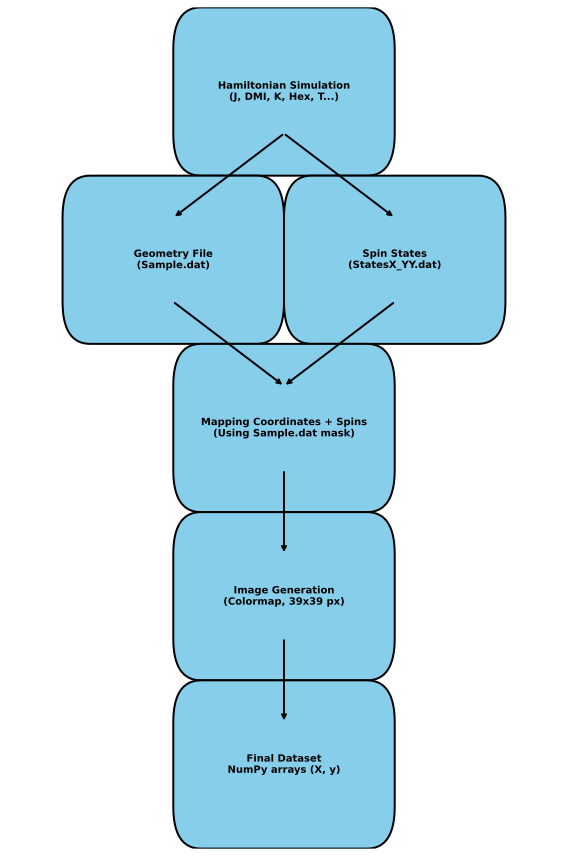
\includegraphics[width=0.7\linewidth]{Figures/pipeline_vertical_branch.pdf}
    \caption{Dataset generation}
    \label{fig:pipeline}
\end{figure}

\subsection{Deep Learning for Parameter Estimation}

Given an image set of spin configurations 
\[
\{ I_n \in \mathbb{R}^{H \times \widetilde{W} \times C} : n \in \mathbb{N} \},
\]
where $H$ and $\widetilde{W}$ denote the image height and width (in our case $H = \widetilde{W} = 39$), and $C$ is the number of color channels ($C = 1$ for grayscale spin maps), the learning task is to infer the underlying Hamiltonian parameters associated with each $n$-th image.  
Formally, let 
\[
\mathbf{y}_n \in \mathbb{R}^P
\]
be the vector of $P$ physical parameters corresponding to image $I_n$ (e.g., temperature $T$, exchange constants $J$, Dzyaloshinskii–Moriya interaction $D$, anisotropy $K$, external field $H_{ex}$).  

The objective is to construct a regression function 
\[
\hat{\mathbf{y}}_n = f_\Theta(I_n),
\]
where $f_\Theta : \mathbb{R}^{H \times \widetilde{W} \times C} \rightarrow \mathbb{R}^P$ is parameterized by deep convolutional neural networks (CNNs), and $\Theta$ denotes the set of trainable parameters.

\paragraph{Network architecture.}  
We employed convolutional neural networks stacking multiple layers of feature extraction, non-linear activations, and pooling operations. At each $l$-th layer ($l \in L$), the transformation is defined as:
\[
F_l = \varphi_l(F_{l-1}) = \sigma_l(W_l \otimes F_{l-1} + b_l),
\]
where $F_{l-1}$ is the input feature map from the previous layer, $W_l \in \mathbb{R}^{\tilde{k}_l \times \tilde{k}_l \times D_{l-1} \times D_l}$ and $b_l \in \mathbb{R}^{D_l}$ are the learnable convolutional weights and biases, $\tilde{k}_l$ is the kernel size, $\otimes$ denotes convolution, and $\sigma_l(\cdot)$ is a non-linear activation function (ReLU). The feature map $F_l \in \mathbb{R}^{H_l \times \widetilde{W}_l \times D_l}$ captures $D_l$ distinct features from the input representation.

The final layers consist of fully connected (dense) layers projecting the high-dimensional feature embedding into the target space of physical parameters:
\[
\hat{\mathbf{y}}_n = f_\Theta(I_n) \in \mathbb{R}^P.
\]

\paragraph{Optimization framework.}  
The trainable parameter set is 
\[
\Theta = \{ W_l, b_l : l \in L \}.
\]  
It is optimized by minimizing the expected loss between ground-truth labels $\mathbf{y}_n$ and predictions $\hat{\mathbf{y}}_n$ across the dataset:
\[
\Theta^* = \arg \min_\Theta \, \mathbb{E} \big[ \mathcal{L}(\mathbf{y}_n, \hat{\mathbf{y}}_n \,|\, \Theta) : \forall n \in \mathbb{N} \big],
\]
where $\mathcal{L} : \mathbb{R}^P \times \mathbb{R}^P \rightarrow \mathbb{R}$ is a regression loss function (Mean Squared Error, Mean Absolute Error, or Symmetric Mean Absolute Percentage Error). The expectation operator accounts for averaging across the training distribution.

\paragraph{Implementation details.}  
In practice, we tested multiple CNN architectures (ResNet50, InceptionV3, EfficientNetB0/B2, DenseNet121), employing transfer learning where possible. DenseNet121 achieved the best trade-off between accuracy and stability, particularly for temperature estimation. Models were trained using backpropagation with the Adam optimizer, early stopping, and batch normalization for regularization.


\subsection{Regression Activation Maps (RAMs) for Interpretability}

To enhance interpretability of the regression models, we adapted the Grad-CAM technique to the estimation of continuous Hamiltonian parameters. While traditional Class Activation Maps (CAMs) are designed for categorical outputs, in our case the target is a real-valued parameter $\hat{y} \in \mathbb{R}$, such as exchange interaction $J$, anisotropy $K$, DMI, or temperature $T$. We therefore define \textit{Regression Activation Maps} (RAMs), which highlight the spatial regions in the input image that contribute most to the prediction of a given continuous parameter.

\paragraph{Computation of RAMs.}  
Given an input image $I$ and a trained CNN model with parameter set $\Theta^*$, the Grad-CAM procedure was modified to incorporate regression loss. For a selected convolutional layer $l$, the activations $F_l \in \mathbb{R}^{H_l \times \widetilde{W}_l \times D_l}$ and the prediction $\hat{y}$ are simultaneously extracted. We define the relevance weights as:

\begin{equation}
\alpha^{(p)}_{ld} = \frac{1}{H_l \cdot \widetilde{W}_l} \sum_{i=1}^{H_l} \sum_{j=1}^{\widetilde{W}_l} \frac{\partial \mathcal{L}(y_\text{real}, \hat{y})}{\partial F_{ld}[i,j]},
\end{equation}

where $\mathcal{L}(y_\text{real}, \hat{y}) = 1 - |y_\text{real} - \hat{y}|$ is the regression-based relevance function, $F_{ld}[i,j]$ is the $(i,j)$ element of the $d$-th feature map at layer $l$, and $\alpha^{(p)}_{ld}$ measures the contribution of this activation to the error with respect to the real value $y_\text{real}$.

The heatmap is then computed as:

\begin{equation}
S^{(p)}_l = \text{ReLU} \left( \sum_{d=1}^{D_l} \alpha^{(p)}_{ld} \, F_{ld} \right),
\end{equation}

and up-sampled via operator $\Lambda : \mathbb{R}^{H_l \times \widetilde{W}_l} \rightarrow \mathbb{R}^{H \times \widetilde{W}}$ to match the input image resolution.

\paragraph{Implementation details.}  
RAMs were generated for multiple convolutional layers of the trained DenseNet121 backbone, including: \texttt{conv2\_block6\_1\_conv}, \texttt{conv3\_block5\_1\_conv}, \texttt{conv3\_block10\_2\_conv}, \texttt{conv4\_block4\_2\_conv}, \texttt{conv4\_block7\_2\_conv}, \texttt{conv4\_block11\_1\_conv}, \texttt{conv4\_block17\_2\_conv}, \texttt{conv5\_block2\_1\_conv}, \texttt{conv5\_block8\_1\_conv}, and \texttt{conv5\_block16\_1\_conv}. For each image in the dataset, a grid was constructed containing the original spin configuration alongside the corresponding RAMs for each selected layer, enabling visual inspection of which regions (e.g., domain walls, vortices, skyrmionic cores) were most influential in the regression.



These measures provide a quantitative framework to validate whether the model is attending to physically meaningful features in the images, bridging the gap between black-box regression predictions and interpretable physical insight.



%%%%% FALTA TEST DE HIPOTESIS PARA VALIDAR MEJOR MODELO.
\section{Experimental Set-Up}\label{sec:experiments}



In this section, we first describe the setup used to evaluate our approach for predicting the parameters of interest. Next, we present and discuss the experimental results.

\subsection{Tested Dataset}\label{sec:Data}

To evaluate the proposed model, we employed two public datasets available on Kaggle: \textbf{KDM DATABASE SPINERS}\footnote{\url{https://www.kaggle.com/datasets/deathperminut/kdm-database-spiners}} and \textbf{MATERIAL SPINNERS DATA}\footnote{\url{https://www.kaggle.com/datasets/deathperminut/material-spinners-data}}. The \textbf{KDM DATABASE SPINERS} dataset, which serves as our primary benchmark, contains a total of 164,212 grayscale images of $39 \times 39$ pixels, stored in \texttt{.npy} format. Each image is associated with a set of Hamiltonian parameters, focusing particularly on temperature (T) and a derived parameter (KDM) that combines anisotropy and Dzyaloshinskii–Moriya interactions. This dataset was synthetically generated to simulate realistic spin textures under thermal variations, offering a comprehensive representation of temperature-driven domain configurations.

The secondary dataset, \textbf{MATERIAL SPINNERS DATA}, complements the first by exploring different physical regimes. It consists of 54,404 images of the same resolution and format, but varies key exchange interaction parameters  along with temperature. This configuration enables the analysis of more intricate spin behaviors and nonlinear interactions among physical constants, enhancing the generalization capabilities of the model. Both datasets share a common labeling scheme, facilitating model training and transferability while covering distinct portions of the Hamiltonian parameter space.

The structure of the dataset follows a Python dictionary format, 
where each key represents a parameter name and its value corresponds 
to an array of data. The available variables are:


\begin{longtable}{ll}
\caption{Description of dataset variables.} \label{tab:variables} \\
\hline
\textbf{Variable} & \textbf{Description} \\
\hline
\endfirsthead
\hline
\textbf{Variable} & \textbf{Description} \\
\hline
\endhead
\texttt{MS}   & Set of images \\
\texttt{Nest} & State number \\
\texttt{L}    & Sample thickness \\
\texttt{rd}   & Sample radius \\
\texttt{So}   & Spin \\
\texttt{T}    & Temperature \\
\texttt{Jex}  & First-neighbor exchange interaction \\
\texttt{Jex2} & Second-neighbor exchange interaction \\
\texttt{Jex3} & Third-neighbor exchange interaction \\
\texttt{Jex4} & Fourth-neighbor exchange interaction \\
\texttt{Kan1} & First magnetocrystalline anisotropy constant \\
\texttt{Kan2} & Second magnetocrystalline anisotropy constant \\
\texttt{KanS} & Surface anisotropy constant \\
\texttt{Hex}  & External magnetic field \\
\texttt{kd}   & Dipolar constant \\
\texttt{KDM}  & Dzyaloshinskii--Moriya interaction \\
\hline
\end{longtable}

Spin configurations based on the Heisenberg model were implemented to reproduce various magnetic structures such as patterns, vortices, helical distributions, and other experimentally observed formations. A nanodisk geometry was selected to extract additional information on edge effects. A radius of 18.3 muc was considered to ensure the occurrence of the second-order magnetic phase transition in magnetization as a function of temperature. The loss of the 2D transition under the Heisenberg model is well known.

Here, $\mathbf{S}$ represents the spin vector, which was set to 1 for normalization. $J_{Nn}$ denotes the exchange constant, where $N = 1, 2, 3, 4$ corresponds to the first to fourth nearest neighbors. $K_{DM_{ij}}^z$ the Dzyaloshinskii-Moriya (DM) constant with interaction up to third neighbors, $h_{\text{Ex}}$ is the external magnetic field, and $K_{\text{An}}$ is the magnetocrystalline anisotropy constant. The variables $\alpha_1$, $\alpha_2$, and $\alpha_3$ denote the direction cosines along the three Cartesian axes. Given the sample geometry, only the in-plane contribution of the Dzyaloshinskii–Moriya (DM) interaction was considered, up to second-nearest neighbors. $J_1$ was fixed at 1~meV per spin pair to define a reference energy scale. The Curie temperature—corresponding to the second-order transition from paramagnetic to ferromagnetic behavior—was set at 15.3~K, assuming no other competing parameters. The remaining interaction strengths were randomly assigned values between $-0.5$ and $0.5$~meV, consistent with values reported in DFT studies for various materials \cite{ref2}.

Simulations began from randomly initialized spin configurations. The temperature was decreased from 20~K to 0.1~K in steps of 0.1~K. The system was evolved using the Metropolis algorithm and the Monte Carlo method, with 20,000 steps per temperature and the last 10,000 used for statistical averaging. For each simulation, 100 runs were executed under similar parameters, each starting from a different random spin configuration.

Some of the physical parameters in the dataset were fixed across the simulations to simplify the experimental setup and reduce the complexity of the modeling task. In particular, variables such as Jex, Jex2, Jex3, Jex4, and kd were kept constant in many of the samples, which is reflected by their near-zero variance. This decision was motivated by the aim of focusing the learning process on more influential or variable quantities such as T, KDM, and the anisotropy constants (Kan1, KanS).


\begin{figure}[htbp!]
    \centering
    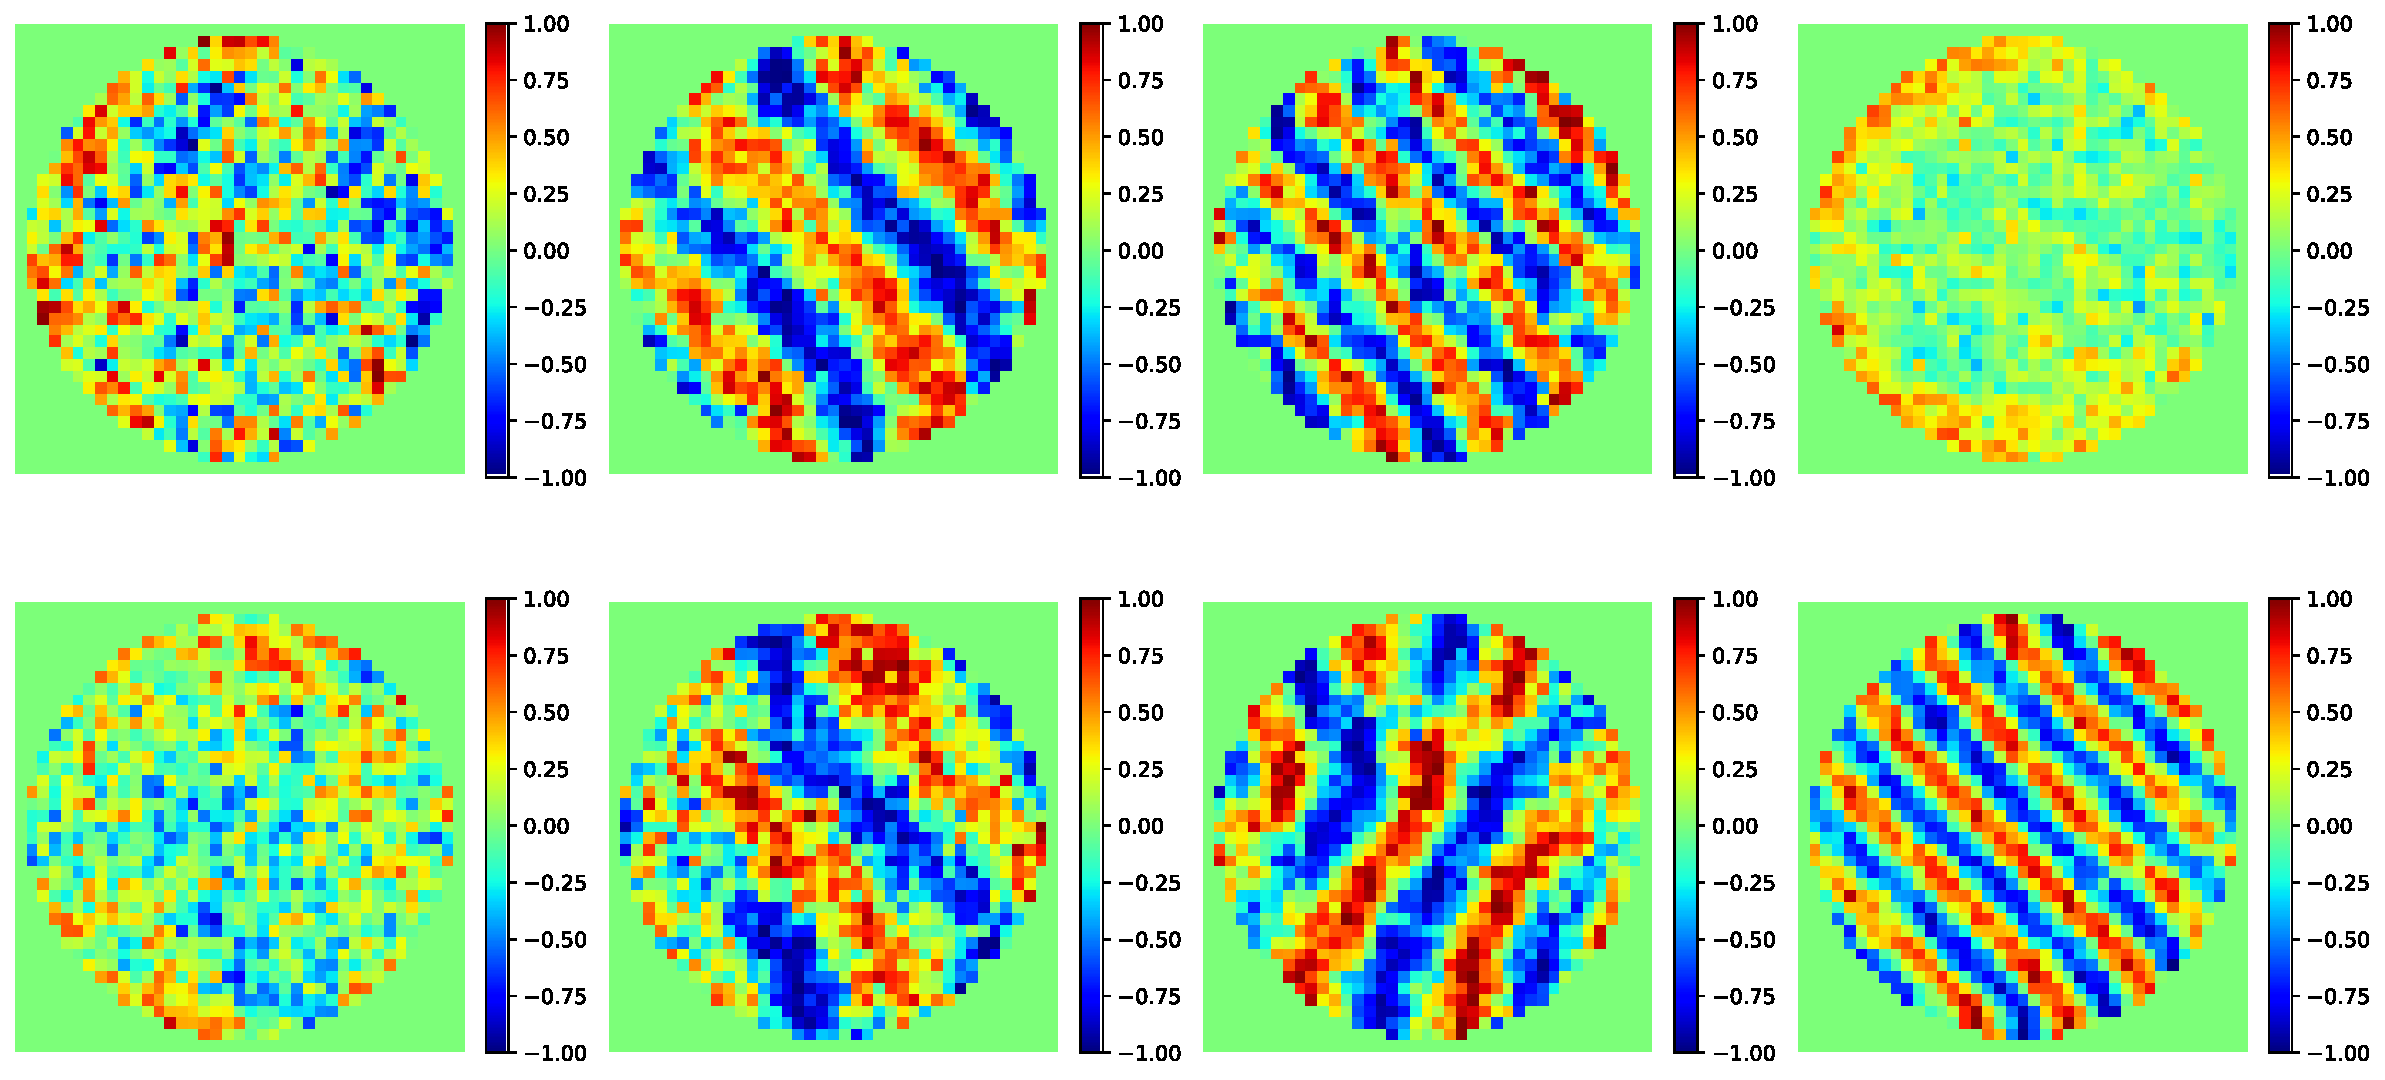
\includegraphics[width=0.85\linewidth]{Figures/imagenes_grid.pdf}
    \caption{KDM Dataset Nanodots States Example }
    \label{fig:kdm_dataset}
\end{figure}

\begin{figure}[htbp!]
    \centering
    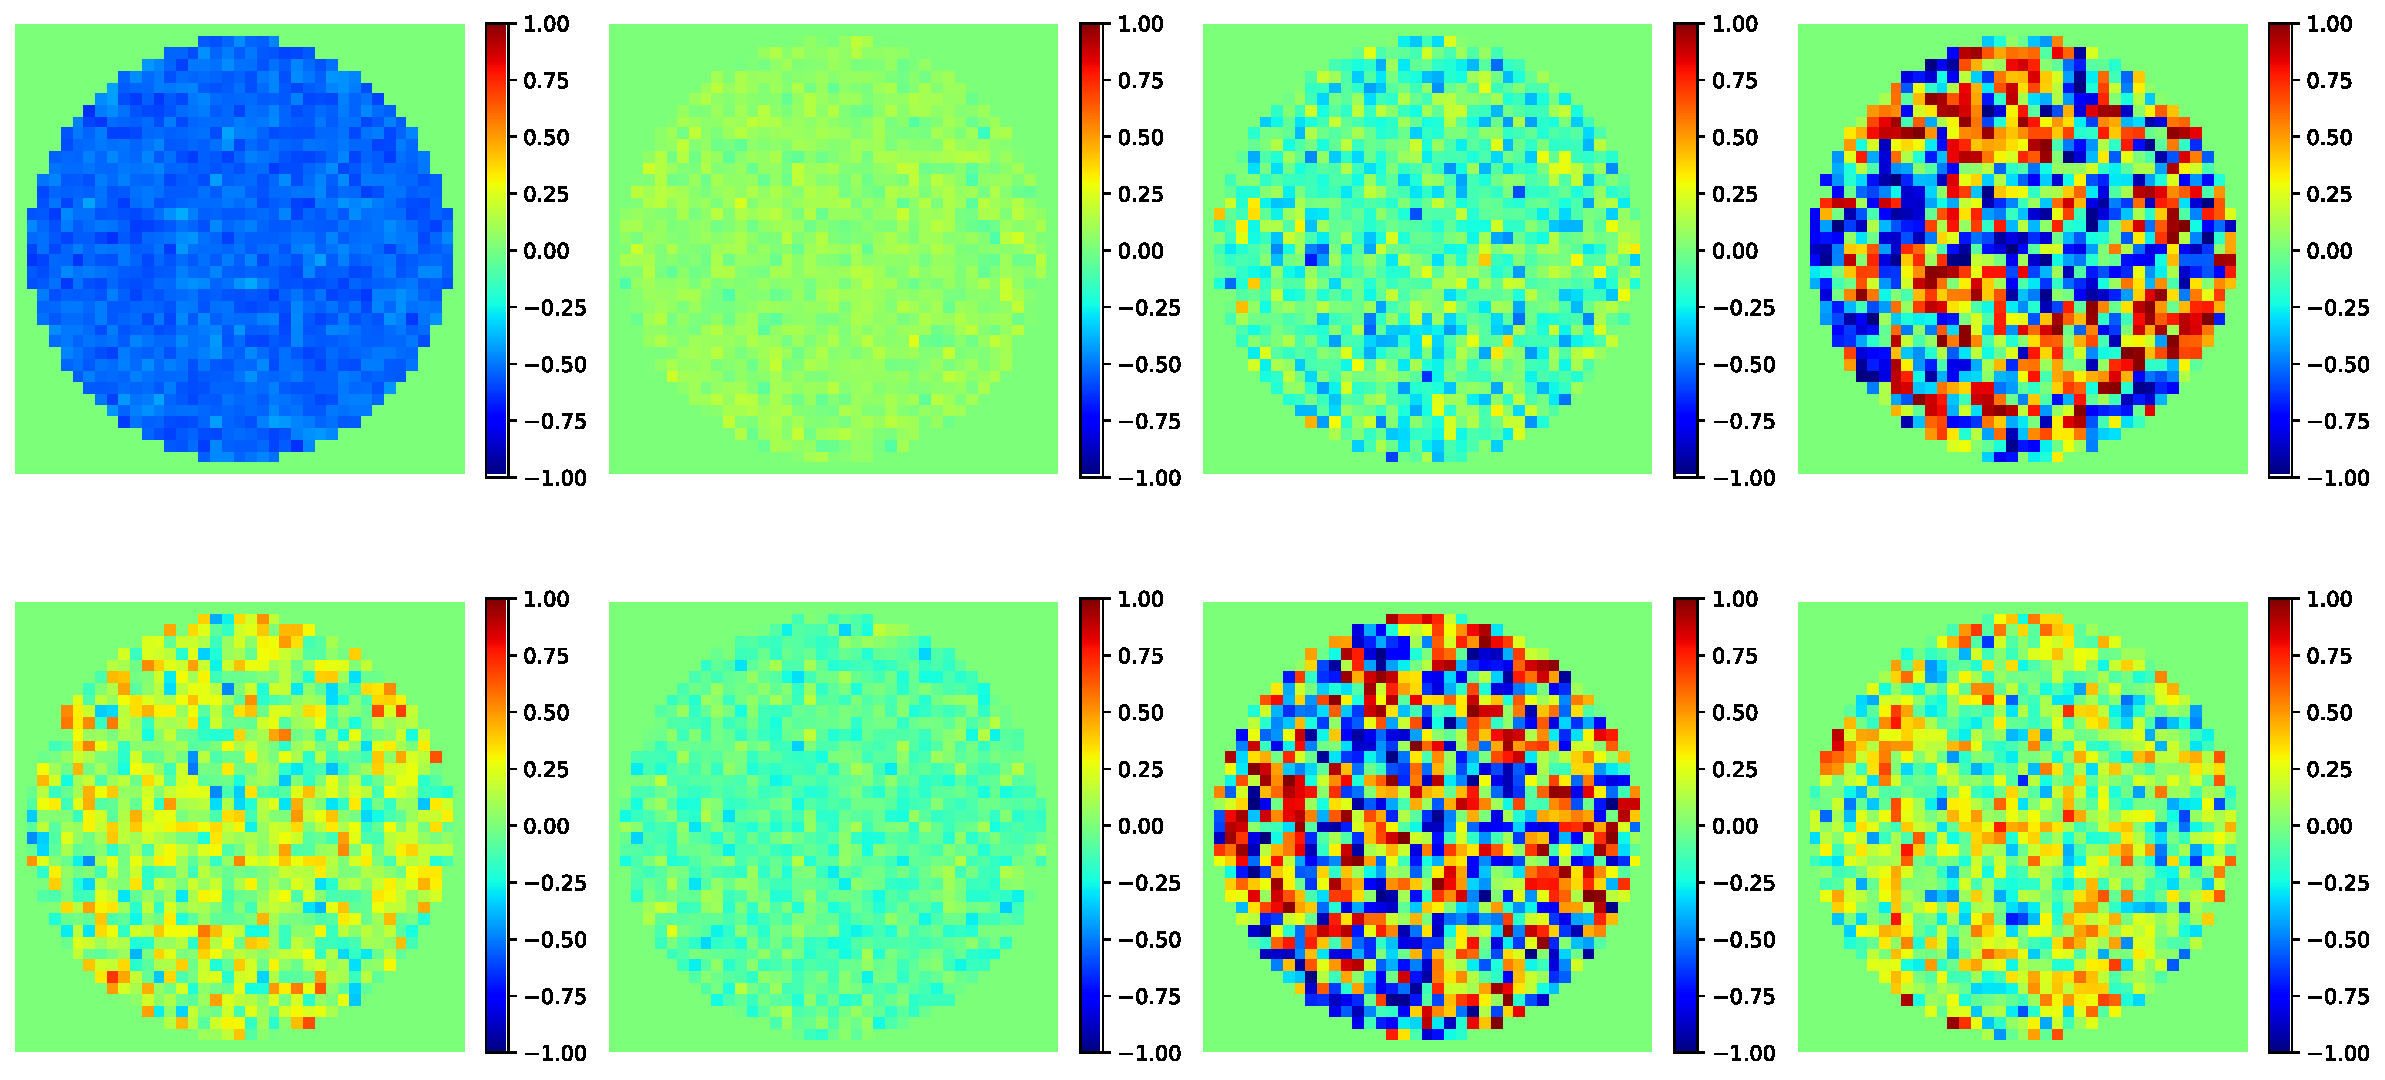
\includegraphics[width=0.85\linewidth]{Figures/imagenes_grid2.pdf}
    \caption{Material Spinner Dataset Nanodots States Example }
    \label{fig:spinner_dataset}
\end{figure}

The distribution of each parameter present in the dataset is shown in Figure~\ref{fig:distribution}. Parameters with nearly uniform distributions across ranges (e.g., \texttt{Kan1}, \texttt{Hex}) indicate that they were sampled broadly, while others with sharp peaks or narrow ranges (e.g., \texttt{rd}, \texttt{kd}) reflect fixed or constrained simulation settings.


\begin{figure}[htbp!]
    \centering
    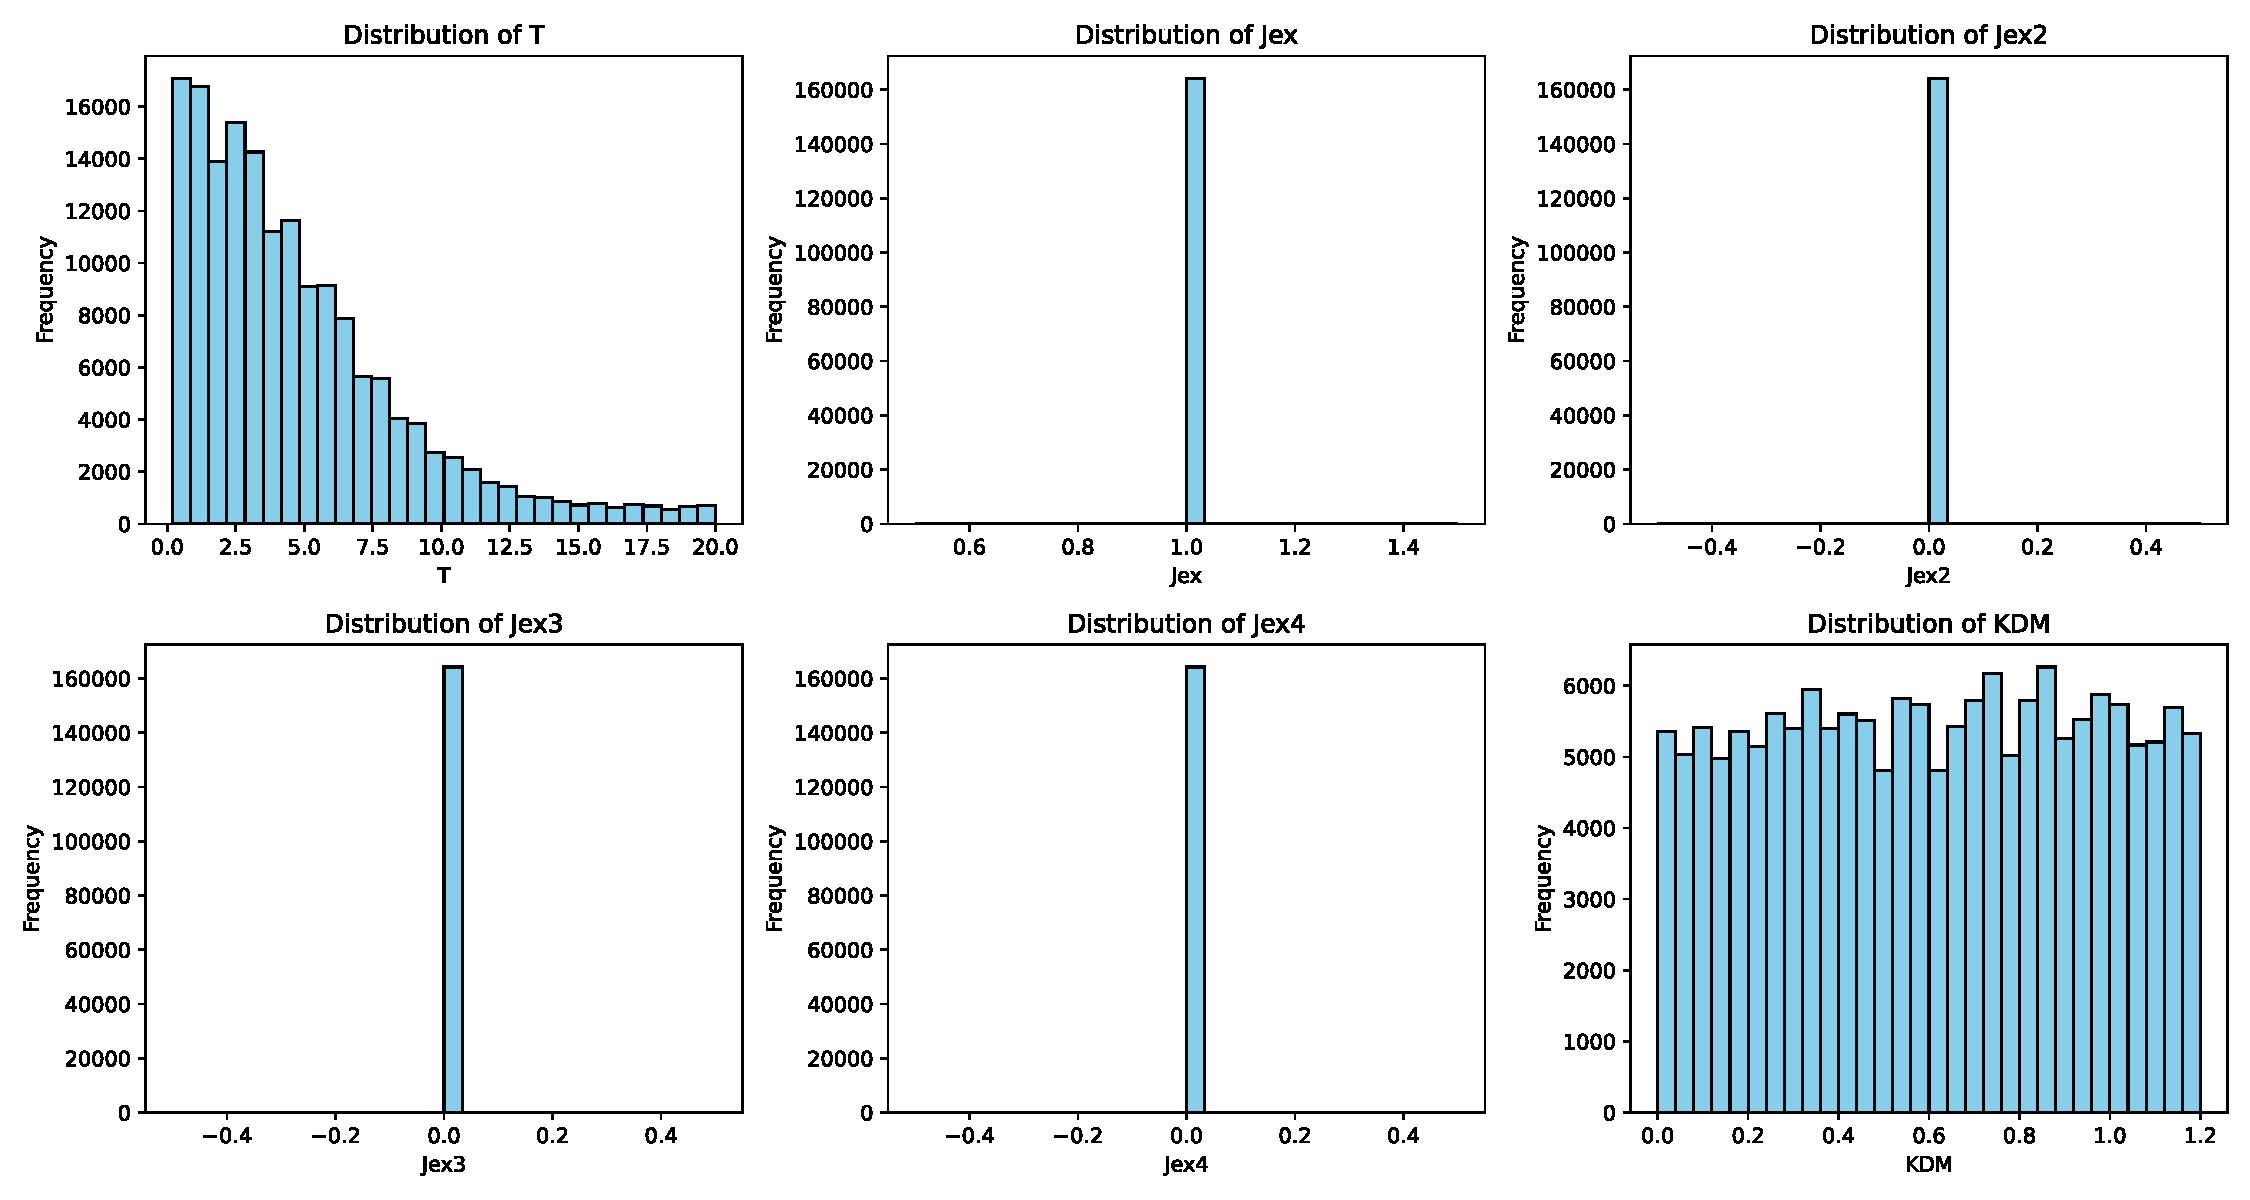
\includegraphics[width=0.85\linewidth]{Figures/distribuciones_parametrosKDM.pdf}
    \caption{Parameter distribution across the full KDM Database }
    \label{fig:distribution_kdm}
\end{figure}


\begin{figure}[htbp!]
    \centering
    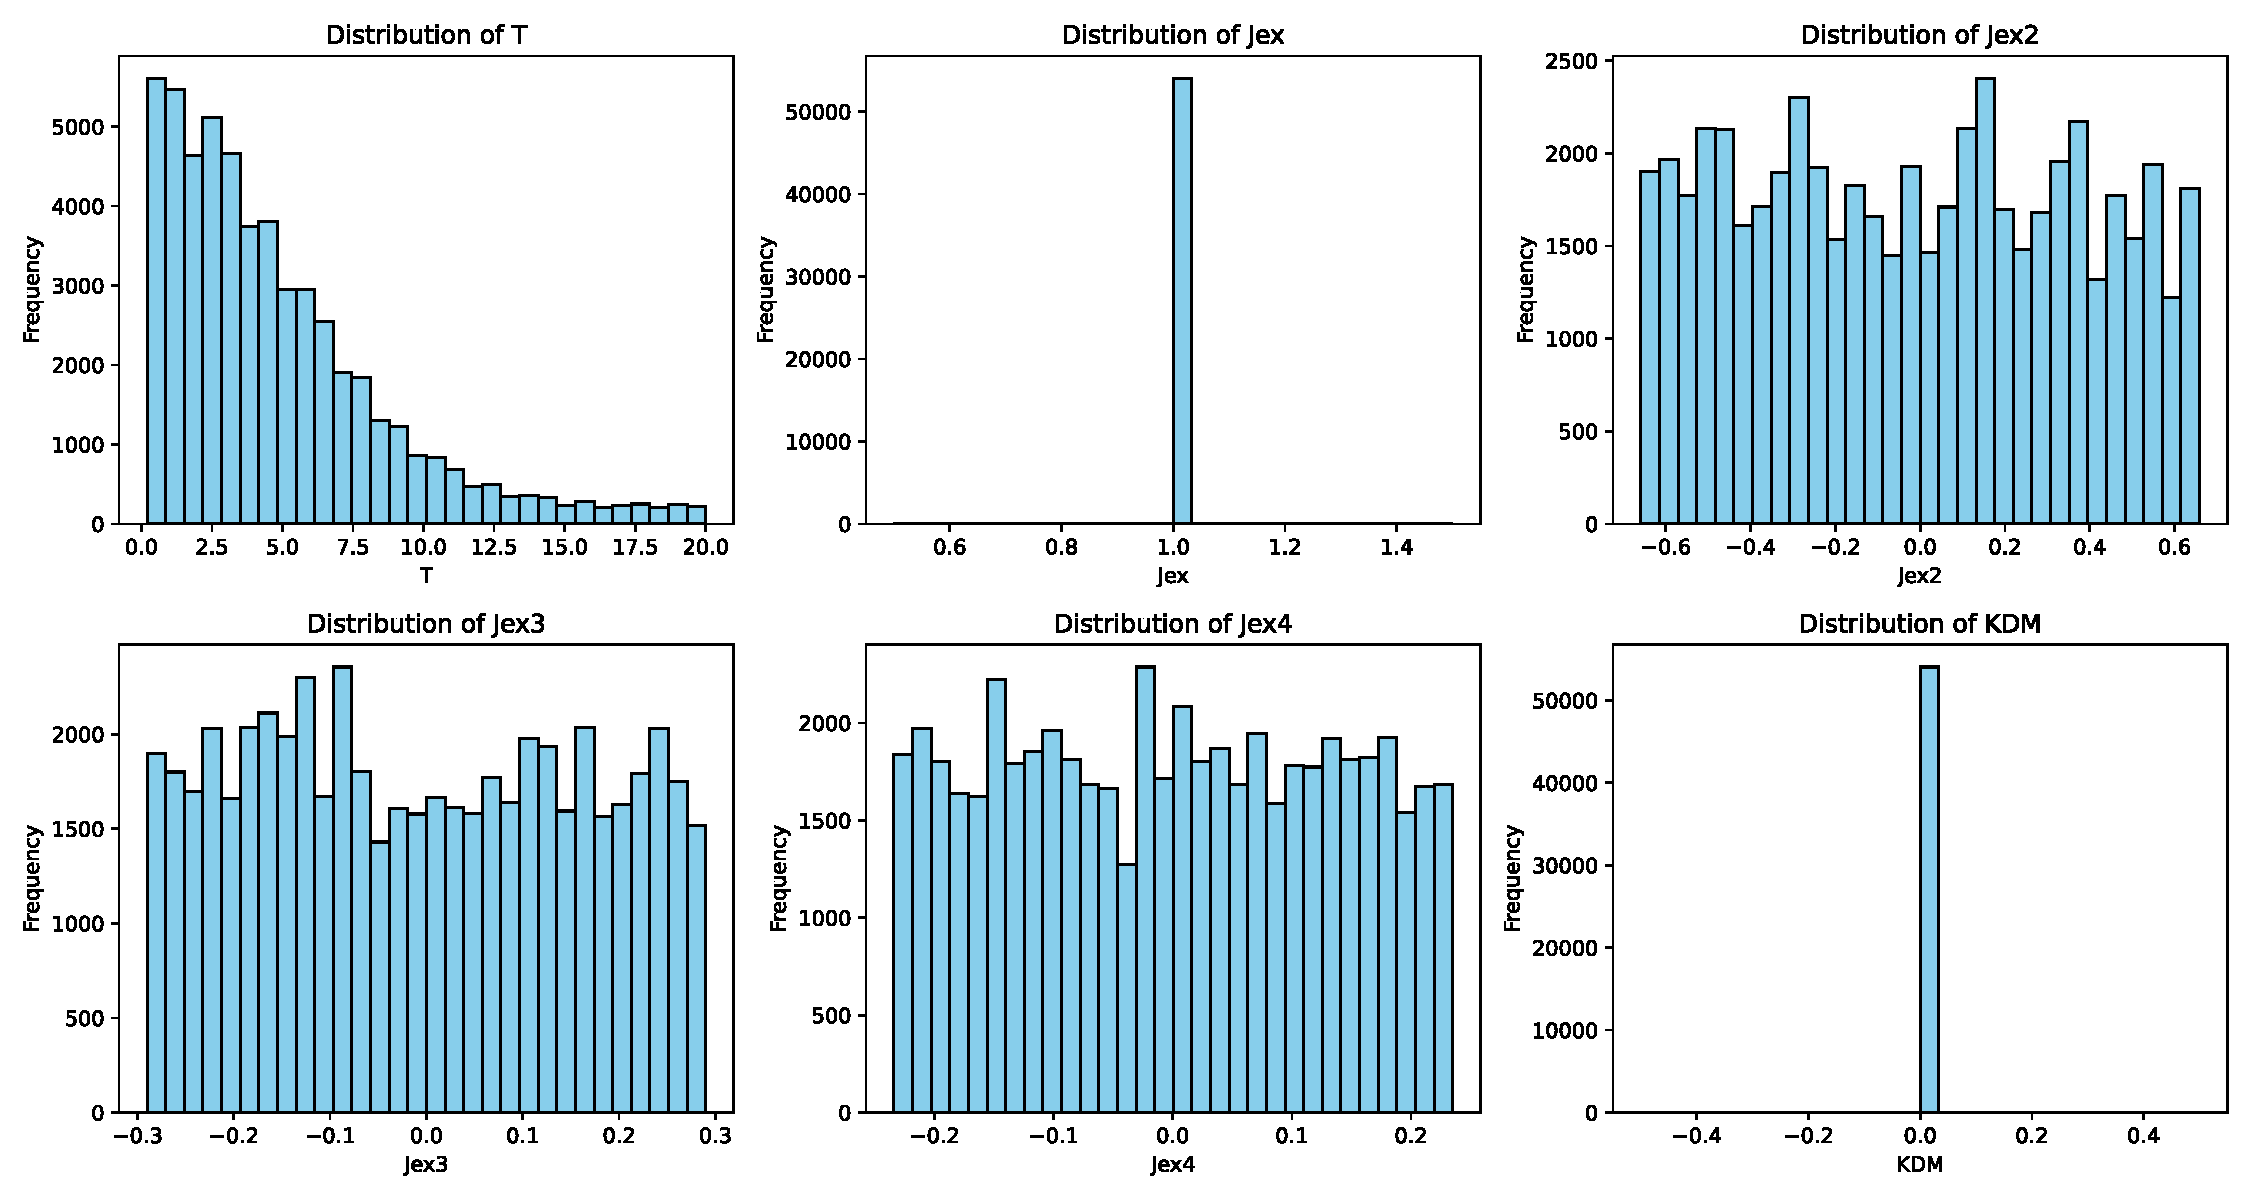
\includegraphics[width=0.85\linewidth]{Figures/distribuciones_parametrosTJex2.pdf}
    \caption{Parameter distribution across the full Material Spinner Database}
    \label{fig:distribution_jex2}
\end{figure}
\FloatBarrier

\subsection{Method Comparison and Training Details}\label{sec:MC}

The task is formulated as a multivariate regression problem (KDM and T of "KDM Database"), where each model takes as input an image representing the material's spin structure and simultaneously predicts multiple physical parameters associated with the sample. Due to computational resource limitations, a representative subset of 50,000 images was selected from the full dataset, ensuring that the original distributions of the physical variables were preserved. The proposed approach is based on transfer learning, leveraging image encoders from state-of-the-art computer vision architectures to extract high-level representations from the spin configurations before performing regression.

\begin{figure}[!h]
\centering
\includegraphics[width=0.75\linewidth]{Figures/Esquema.png}
\caption{Model design}
\label{fig:distribution}
\end{figure}
\FloatBarrier

In this approach, we utilized pretrained weights from ImageNet, allowing the model to benefit from learned representations and speed up convergence during training. The final layers of the original architectures were replaced with regression-specific layers, enabling the model to output a multivariate regression corresponding to the target physical properties.

The architectures implemented, all available in TensorFlow, are summarized in The architectures implemented, all available in TensorFlow, 
are summarized in Table~\ref{tab:architectures}.

\begin{longtable}{ll}
\caption{Deep learning architectures used in this study.} \label{tab:architectures} \\
\hline
\textbf{Model} & \textbf{Description / Notes} \\
\hline
\endfirsthead

\hline
\textbf{Model} & \textbf{Description / Notes} \\
\hline
\endhead

DenseNet121    & Dense Convolutional Network, 121 layers \\
ResNet50       & Residual Network, 50 layers \\
Inception      & Inception v3 architecture \\
EfficientNetB0 & EfficientNet baseline model (lightweight) \\
EfficientNetB2 & Scaled EfficientNet variant (deeper than B0) \\
\hline
\end{longtable}

All convolutional models were trained using the Adam optimizer. The mean squared error (MSE) was used as the primary loss function:

\begin{equation}
\text{MSE} = \frac{1}{n} \sum_{i=1}^n (y_i - \hat{y}_i)^2
\end{equation}

Additionally, the mean absolute error (MAE) was employed as a complementary evaluation metric:

\begin{equation}
\text{MAE} = \frac{1}{n} \sum_{i=1}^n |y_i - \hat{y}_i|
\end{equation}

This optimization and evaluation scheme was consistently applied across all explored architectures.

The deep learning models were trained using a train-test split strategy, where 80 percent of the data was allocated for training (training set), 10 percent for validation (validation set), and 10 percent for testing (test set). Prior to training, the data was normalized using the MinMaxScaler technique from the scikit-learn library to ensure consistent feature scaling. The models were trained for 10 epochs using a A100 GPU on Google Colab, leveraging its high computational power to accelerate training.

The performance of each model was evaluated on the test set using two quantitative metrics: the coefficient of determination (R\textsuperscript{2}) and the symmetric mean absolute percentage error (SMAPE):

\begin{equation}
R^2 = 1 - \frac{\sum_{i=1}^{n} (y_i - \hat{y}i)^2}{\sum{i=1}^{n} (y_i - \bar{y})^2}
\end{equation}

\begin{equation}
\text{SMAPE} = \frac{100}{n} \sum_{i=1}^n \frac{|y_i - \hat{y}_i|}{(|y_i| + |\hat{y}_i|)/2}
\end{equation}

\textbf{R\textsuperscript{2}} measures how well the predicted values fit the actual values, while \textbf{SMAPE} provides a percentage-based error evaluation, making it robust to both over- and under-predictions.

To analyze feature representations, we evaluated the distribution of the predicted parameters across different layers of each CNN using the Uniform Manifold Approximation and Projection (UMAP) technique. Let  denote the activations of a given convolutional layer . UMAP projects these high-dimensional activations into a lower-dimensional space  for visualization:

\begin{equation}
Z_l = \text{UMAP}(X_l), \quad X_l \in \mathbb{R}^{n \times d_l}, Z_l \in \mathbb{R}^{n \times 2}
\end{equation}

This allowed us to observe how the embeddings evolve and structure with respect to physical parameters across different network depths.



Finally, we proposed a passive interpretability method for regression problems based on Class Activation Maps (CAMs), which we call Regression Activation Maps (RAMs). To quantify the relevance of regions with respect to the prediction error, we defined a gradient weighting scheme proportional to prediction accuracy:

\begin{equation}
\text{loss} = 1 - |y_i - \hat{y}_i|
\end{equation}

These loss is used in the gradient-based activation computation, highlighting the spatial regions in the input image that contribute most to accurate predictions. This enhances interpretability and provides a more physics-informed visualization of model attention in regression tasks.












\section{Results and Discussion}\label{sec:results}

To assess the predictive performance of the models across the selected physical parameters, we report both the Symmetric Mean Absolute Percentage Error (SMAPE) and the coefficient of determination ($R^2$). Figure~\ref{fig:metrics} summarizes the results obtained for the two most relevant target variables, KDM and T, using five different convolutional encoder architectures: DenseNet121, ResNet50, InceptionV3 and EfficientNetB2. These metrics provide complementary perspectives on model accuracy and generalization. Lower SMAPE values indicate better agreement between predictions and ground truth, while higher $R^2$ values reflect improved explained variance. The figure highlights significant differences in performance across models, underscoring the impact of architecture selection on regression quality for complex physical systems.
\\
\\

\begin{figure}[htbp!]
    \centering
    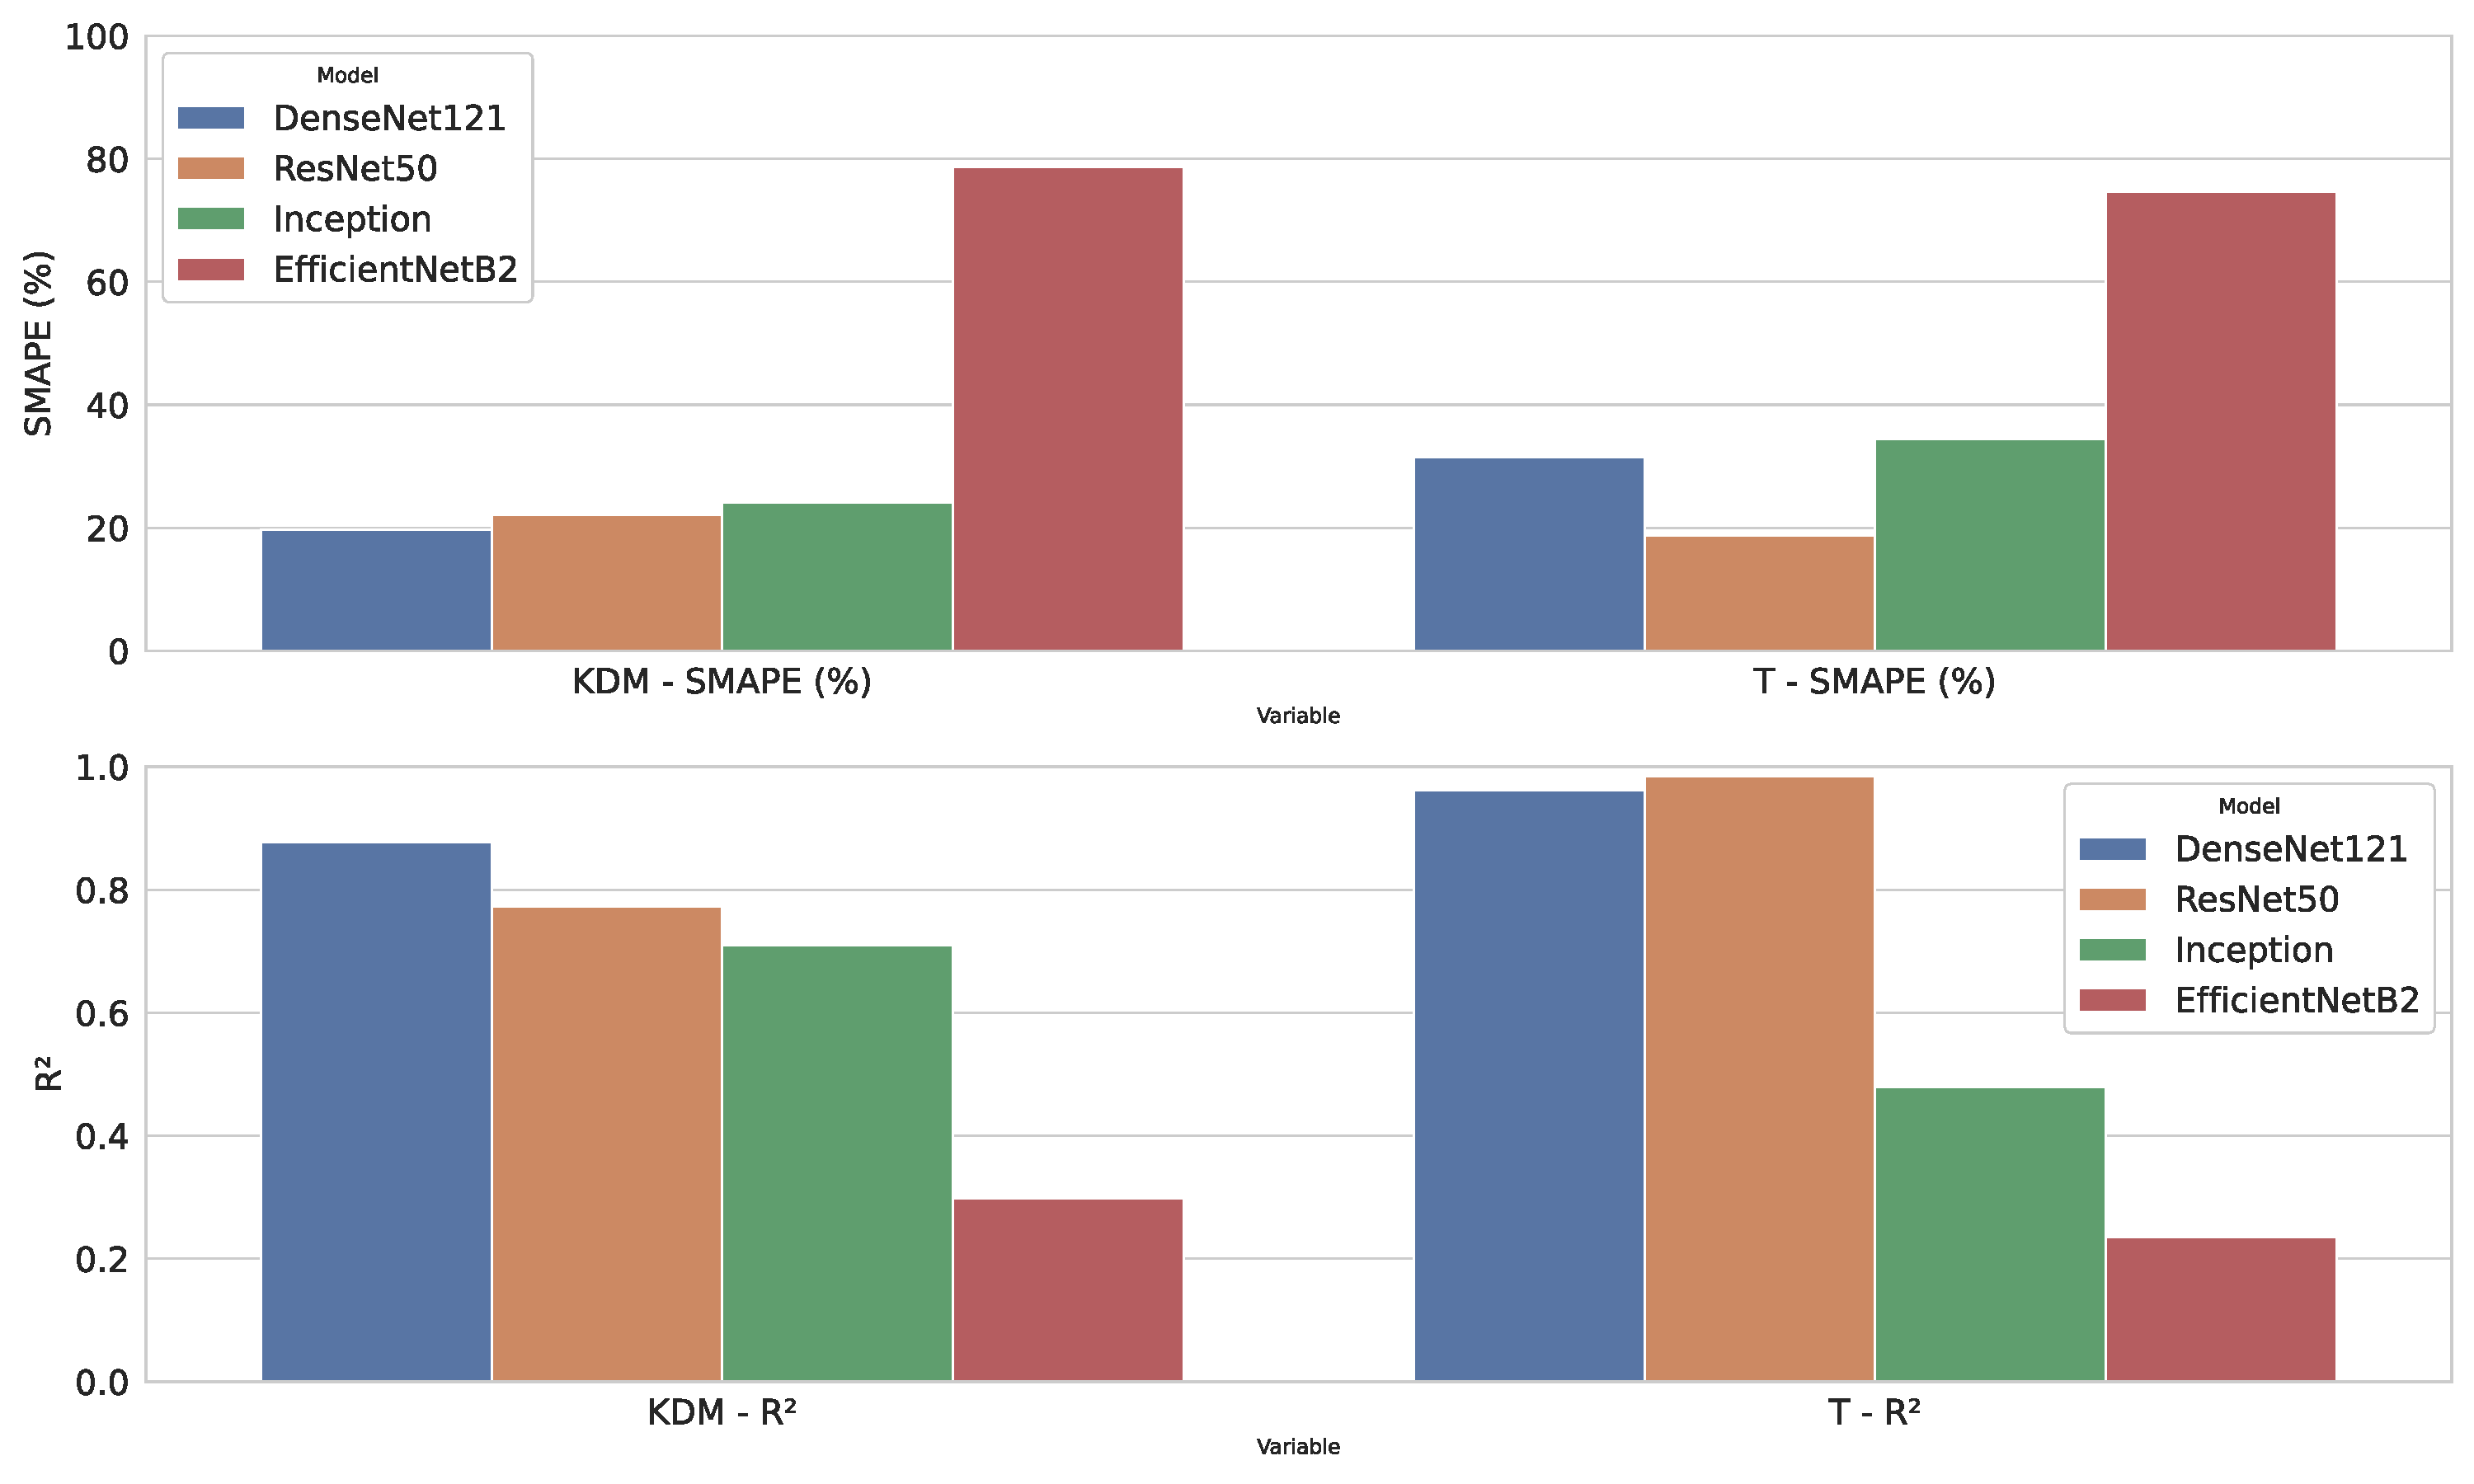
\includegraphics[width=0.95\linewidth]{Figures/comparacion_modelos_separados_KDM.pdf}
    \caption{R2 - SMAPE (KDM Database)}
    \label{fig:comparison_kdm}
\end{figure}
\FloatBarrier
\begin{figure}[htbp!]
    \centering
    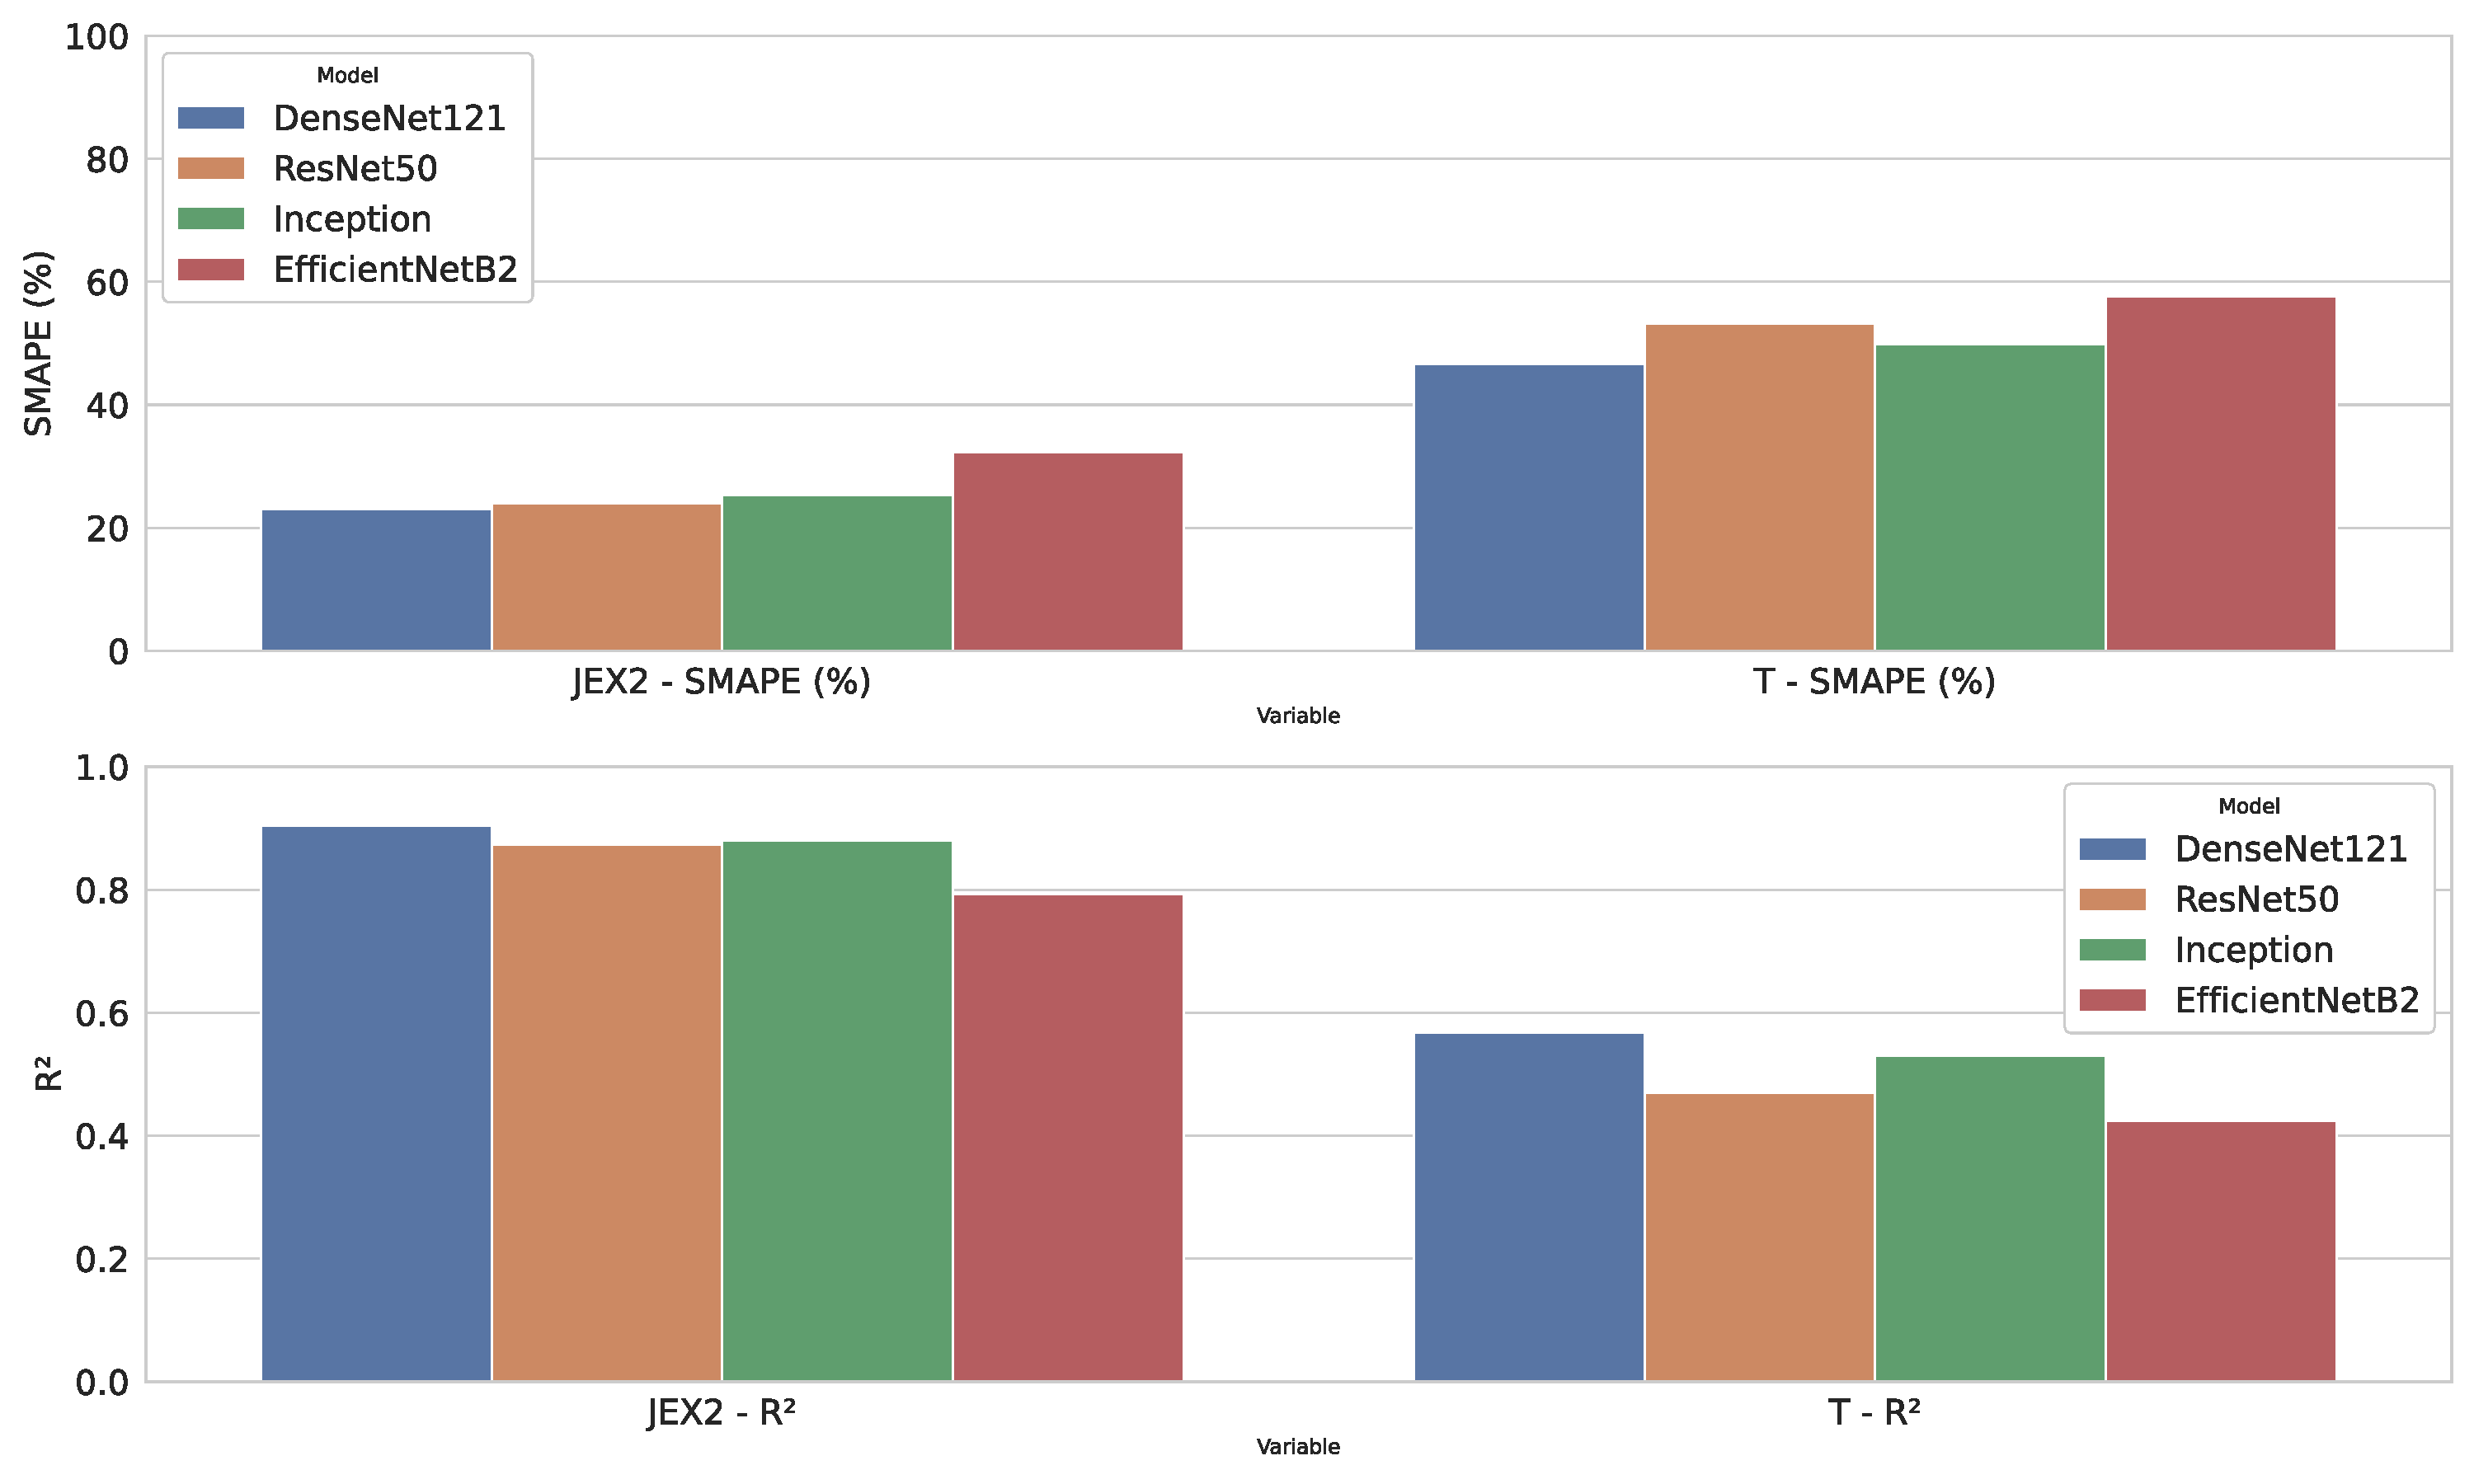
\includegraphics[width=0.95\linewidth]{Figures/comparacion_modelos_separados_JEX2.pdf}
    \caption{R2 - SMAPE (Material Spinner Database)}
    \label{fig:comparison_jex2}
\end{figure}
\FloatBarrier


%\begin{table}[htbp!]
%\centering
%\caption{Ranking based on $R^2$ (KDM Database)}
%\begin{tabular}{|l|c|c|}
%\hline
%\textbf{Model}       & \textbf{T - $R^2$ Rank} & \textbf{KDM - $R^2$ Rank} \\
%\hline
%ResNet50             & 1 & 2 \\
%DenseNet121          & 2 & 1 \\
%Inception            & 3 & 3 \\
%EfficientNetB2       & 4 & 4 \\
%EfficientNetB0       & 5 & 5 \\
%\hline
%\end{tabular}
%\label{tab:ranking_r2}
%\end{table}


%\begin{table}[htbp!]
%\centering
%\caption{Ranking based on SMAPE \% (KDM Database)}
%\begin{tabular}{|l|c|c|}
%\hline
%\textbf{Model}       & \textbf{T - SMAPE Rank} & \textbf{KDM - SMAPE Rank} \\
%\hline
%ResNet50             & 1 & 2 \\
%DenseNet121          & 2 & 1 \\
%Inception            & 3 & 3 \\
%EfficientNetB2       & 4 & 4 \\
%EfficientNetB0       & 5 & 5 \\
%\hline
%\end{tabular}
%\label{tab:ranking_smape}
%\end{table}
%\FloatBarrier



Among the two physical parameters of interest—temperature (\textit{T}) and the Dzyaloshinskii–Moriya interaction magnitude (\textit{KDM})—the latter plays a more critical role in governing the magnetic behavior and stability of spin textures. Consequently, our analysis places greater emphasis on accurately modeling and interpreting \textit{KDM}. While some architectures showed slightly better performance in predicting \textit{T}, DenseNet121 consistently achieved the best balance across both variables and exhibited the lowest SMAPE and highest $R^2$ for \textit{KDM}. For this reason, DenseNet121 was selected for further analysis and interpretation, particularly in understanding the learned representations and their relation to the underlying physical features.
\\


DenseNet (Densely Connected Convolutional Networks) is a convolutional neural network (CNN) architecture characterized by its innovative approach of dense connections between layers. Unlike traditional networks such as ResNet, which employ residual connections (skip connections) where the outputs of previous layers are added to subsequent layers, DenseNet uses a concatenation strategy for the activations of all previous layers. This means that each layer within a dense block receives as input not only the output of the previous layer but all prior outputs within that block. This dense connectivity allows the model to better leverage the features learned by earlier layers, improving the efficiency of feature representation reuse and reducing the need for additional parameters.
\\

One of the most significant advantages of DenseNet is that, due to this feature reuse, the network has greater parameter efficiency compared to other traditional CNN models like ResNet. While DenseNet can be deeper than ResNet, its architecture allows for the training of larger networks without a significant increase in parameters, making it a model less prone to overfitting and more suitable for complex tasks. Additionally, by facilitating better gradient flow during training, DenseNet mitigates the vanishing gradient problem, which can hinder the training of deep networks. In summary, the combination of dense connections, parameter efficiency, and improved gradient flow makes DenseNet a powerful and effective choice for computer vision tasks, overcoming the limitations of models like ResNet and other traditional approaches in convolutional neural networks.

\begin{figure}[htbp!]
\centering
\includegraphics[width=0.9\linewidth]{Figures/Densenet_diagram_V2.png}
\caption{DenseNet Arquitecture }
\label{fig:sketch}
\end{figure}
\FloatBarrier

\begin{figure}[!h]
\centering
\includegraphics[width=0.85\linewidth]{Figures/REGRESION_DENSENET_RESULTS.png}
\caption{Estimation DensetNet Results KDM Database}
\label{fig:distribution}
\end{figure}
\FloatBarrier

%%% DEFINIR LA PALETA DE COLORES GENERAL DEL SEGUNDO DATASET. --CHECK
%% ENTRENAMIENTO INDEPENDIENTE EN CADA SET DE DATOS --CHECK
%% SOLOMANETE EN EL EJE Z. NO TENIA RELACIÓN PERO HICIMOS OTRO TEST
%%% SOLO HAY INFORMACIÓN EN EL EJE Z NO APORTA EL RESTO. -- HICIMOS TEST 
%%% 


While DenseNet121 provides accurate predictions for the variable \textit{T}, the \textit{KDM} estimations show greater dispersion, especially at intermediate and high values. This is mainly due to the increased disorder in spin configurations near the Curie temperature, where magnetic order is lost, making the prediction of \textit{KDM} inherently more challenging.


\begin{figure}[htbp!]
\centering
\includegraphics[width=0.85\linewidth]{Figures/TvsKDM.png}
\caption{Visual inspection of spin configurations over the KDM space conditioned on temperature. Reliable magnetic structures are observed for $T < 10$~K. Above this range, thermal fluctuations dominate and reduce prediction reliability.}
\label{fig:kdm_temp_scatter}
\end{figure}
\FloatBarrier

To further validate the hypothesis that the increased prediction error in \textit{KDM} is associated with the loss of magnetic order near the Curie temperature, we performed an additional analysis by filtering the test set to include only those states with temperature values greater than 10~K. This threshold corresponds to the regime in which spin configurations begin to lose coherence due to thermal agitation, making the estimation of KDM more challenging. By isolating this subset, we aim to quantify and visualize how the deterioration of magnetic structure in high-temperature states affects the model’s ability to infer reliable values for the Dzyaloshinskii–Moriya interaction.

%%% LAYER MAP REGRESIÓN ACTIVATION MAPs.
%%% REVISAR LAS BASES DE DATOS DE TAMBIEN LOS MAPAS DE ACTIVACIÓN.

\begin{figure}[htbp!]
\centering
\includegraphics[width=0.75\linewidth]{Figures/KDM_T_ESTIMATIONv2.png}
\caption{Model estimation performance for \textit{KDM} after filtering the test set to include only states with temperature values $T > 10$~K. The increased dispersion and deviation from the identity line reflect the reduced reliability of \textit{KDM} predictions in the high-temperature regime, where thermal fluctuations disrupt magnetic ordering near the Curie point.}
\label{fig:kdm_scatter}
\end{figure}
\FloatBarrier

% PARRAFO PARA COMPARAR LA PREDICCIÓN DE LA TEMPERATURA EN LA OTRA BASE DE DATOS COMPARANDO LA GENERALIZACIÓN
To address the generality and complexity of the Hamiltonian model, we evaluate the performance of our best-performing model, \textbf{DenseNet121}, in a cross-dataset prediction scenario. Specifically, we train the model using the \textbf{KDM DATABASE SPINERS} dataset, where the magnetic parameter $KDM$ is explicitly defined and temperature is varied, and subsequently test it on the \textbf{MATERIAL-SPINNER-DATASET} . In this secondary dataset, $KDM$ remains constant while parameters such as $J_{ex2}$, $J_{ex3}$, and $J_{ex4}$ are varied alongside temperature. The target variable for this generalization task is temperature ($T$), as it is the only common varying parameter across both datasets. Our working hypothesis is that a sufficiently generalizable model should be capable of capturing latent similarities between spin domain configurations—even under slightly different Hamiltonian formulations—and thus achieve reasonable estimation accuracy on unseen variations. This approach allows us to explore the model's robustness and adaptability to different physical regimes within the same theoretical framework.

\begin{figure}[htbp!]
\centering
\includegraphics[width=0.75\linewidth]{Figures/Cross.png}
\caption{Cross-dataset evaluation setup}
\end{figure}
\FloatBarrier



To better understand how the DenseNet121 model encodes physical information throughout its layers, we conducted a layer-wise analysis using Uniform Manifold Approximation and Projection (UMAP). This dimensionality reduction technique enables the visualization of high-dimensional activation spaces in two dimensions. We extracted intermediate activations from four representative convolutional layers and projected them using UMAP. Each resulting embedding was colored according to either the temperature (\textit{T}) or the Dzyaloshinskii–Moriya interaction magnitude (\textit{KDM}), as shown in Figures~\ref{fig:umap_temp} and~\ref{fig:umap_kdm}, respectively. These visualizations reveal how the internal representations evolve with depth in the network and how effectively they organize around the target variables. Notably, deeper layers exhibit a more structured and gradual separation of patterns, particularly with respect to \textit{T}, while the embeddings colored by \textit{KDM} show greater variability and complexity, consistent with its more challenging estimation.



\begin{figure}[htbp!]
\centering
\includegraphics[width=0.85\linewidth]{Figures/UMAP_T.png}
\caption{UMAP projections of intermediate activations from DenseNet121, colored by temperature (\textit{T}). A clear separation emerges in deeper layers, indicating strong internal encoding of thermal behavior.}
\label{fig:umap_temp}
\end{figure}
\FloatBarrier

\begin{figure}[htbp!]
\centering
\includegraphics[width=0.85\linewidth]{Figures/UMAP_KDM.png}
\caption{UMAP projections of intermediate activations from DenseNet121, colored by Dzyaloshinskii–Moriya interaction (\textit{KDM}). The representations are less linearly separable, suggesting increased difficulty in predicting this parameter.}
\label{fig:umap_kdm}
\end{figure}
\FloatBarrier

To further explore how the model internally organizes the data in its final latent representation, we extracted the activations from the last convolutional layer of DenseNet121—immediately preceding the regression output—and projected them into a 2D space using UMAP. In this visualization, shown in Figure~\ref{fig:latent_space_kdm}, each point corresponds to a sample in the latent space and is colored according to its true \textit{KDM} value. Additionally, representative input spin configuration images are overlaid at their respective locations in the embedding. This composite visualization allows us to qualitatively assess how the model clusters similar magnetic states and how well these clusters align with variations in \textit{KDM}. A smoother spatial gradient or continuity in color within regions would suggest a stronger correlation between latent structure and the target variable, whereas higher dispersion and abrupt transitions may indicate increased difficulty in estimating \textit{KDM}.

\begin{figure}[htbp!]
\centering
\includegraphics[width=0.85\linewidth]{Figures/UMAP_IMAGE_KDM.png}
\caption{UMAP projections of intermediate activations from DenseNet121, colored by Dzyaloshinskii–Moriya interaction (\textit{KDM}). The representations are less linearly separable, suggesting increased difficulty in predicting this parameter.}
\label{fig:umap_kdm}
\end{figure}
\FloatBarrier

Following the training phase, the best-performing model—DenseNet121—was selected for a detailed interpretability analysis. To identify the most relevant regions in the input images that contributed to the model’s performance in regression, we applied Class Activation Maps (CAMs) as a post hoc explainability technique. This analysis focused specifically on the prediction of the magnetic parameter KDM, which exhibited high relevance in prior evaluations. To examine the spatial contribution patterns across different value ranges of KDM, the test dataset was stratified into five groups based on predefined intervals of KDM values. CAMs were then computed for representative samples within each group, enabling the identification of feature map activations that most influenced the regression outcome. This approach allowed us to explore whether distinct regions or features within the magnetic domain images were more influential in different KDM value ranges, offering insights into how the model adapts its attention across the spectrum of this parameter.


\begin{figure}[htbp!]
\centering
\includegraphics[width=0.8\linewidth]{Figures/Ranges.png}
\caption{Ranges for KDM interpretability}
\label{fig:umap_kdm}
\end{figure}
\FloatBarrier

\begin{figure}[htbp!]
    \centering
    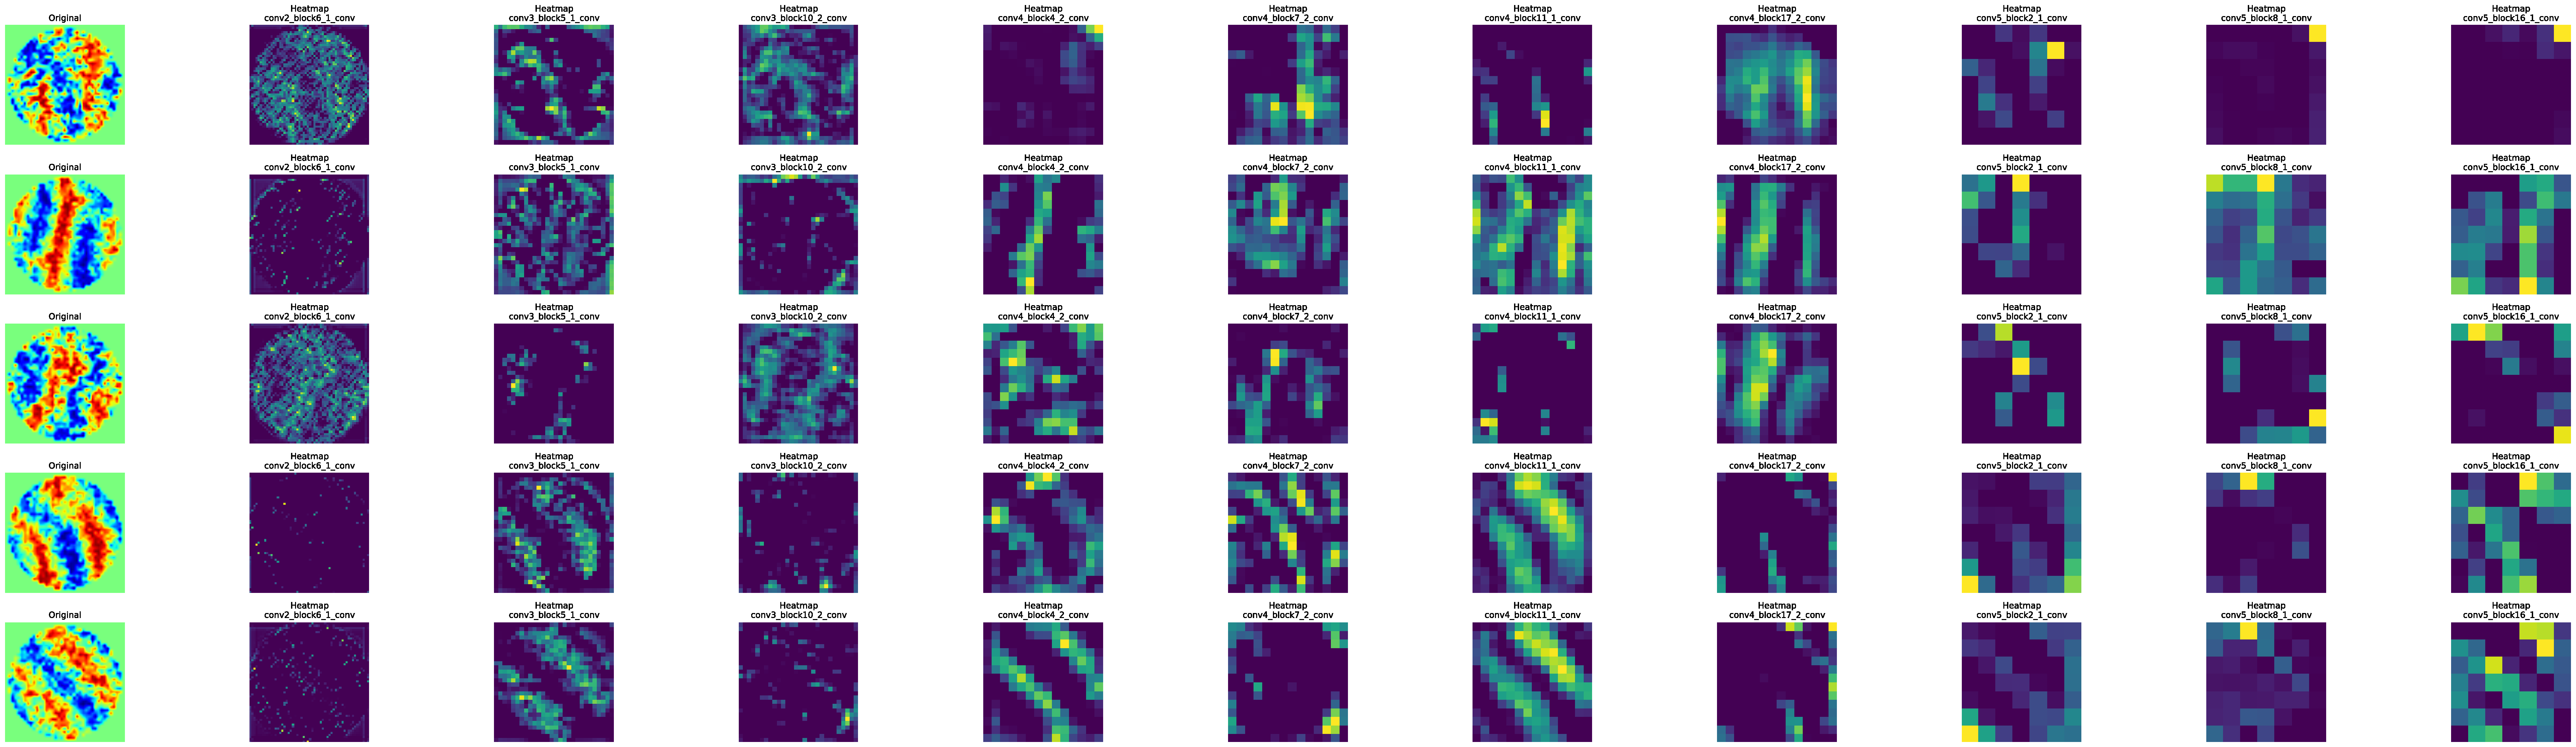
\includegraphics[width=0.85\linewidth]{Figures/gradcam_1.pdf}
    \caption{ Activations maps for domains states DenseNet }
    \label{fig:gradcam_activation}
\end{figure}
\FloatBarrier

To quantitatively assess the contribution of each convolutional layer to the regression task across different ranges of the KDM parameter, we computed the cumulative activation of the CAMs per layer and per KDM value group. Specifically, for each of the five predefined KDM ranges, we aggregated the activation maps generated by the model across all test images belonging to that range. This cumulative analysis was performed layer-wise, allowing us to identify which layers exhibited higher overall activation intensity for each KDM interval. By comparing these cumulative responses, we aimed to reveal which stages of the network architecture were most sensitive or informative for predicting low, medium, and high KDM values. This approach provided a layer-level interpretability framework, highlighting how different levels of feature abstraction contributed to the model's performance in specific value domains of the target parameter.

\begin{figure}[htbp!]
    \centering
    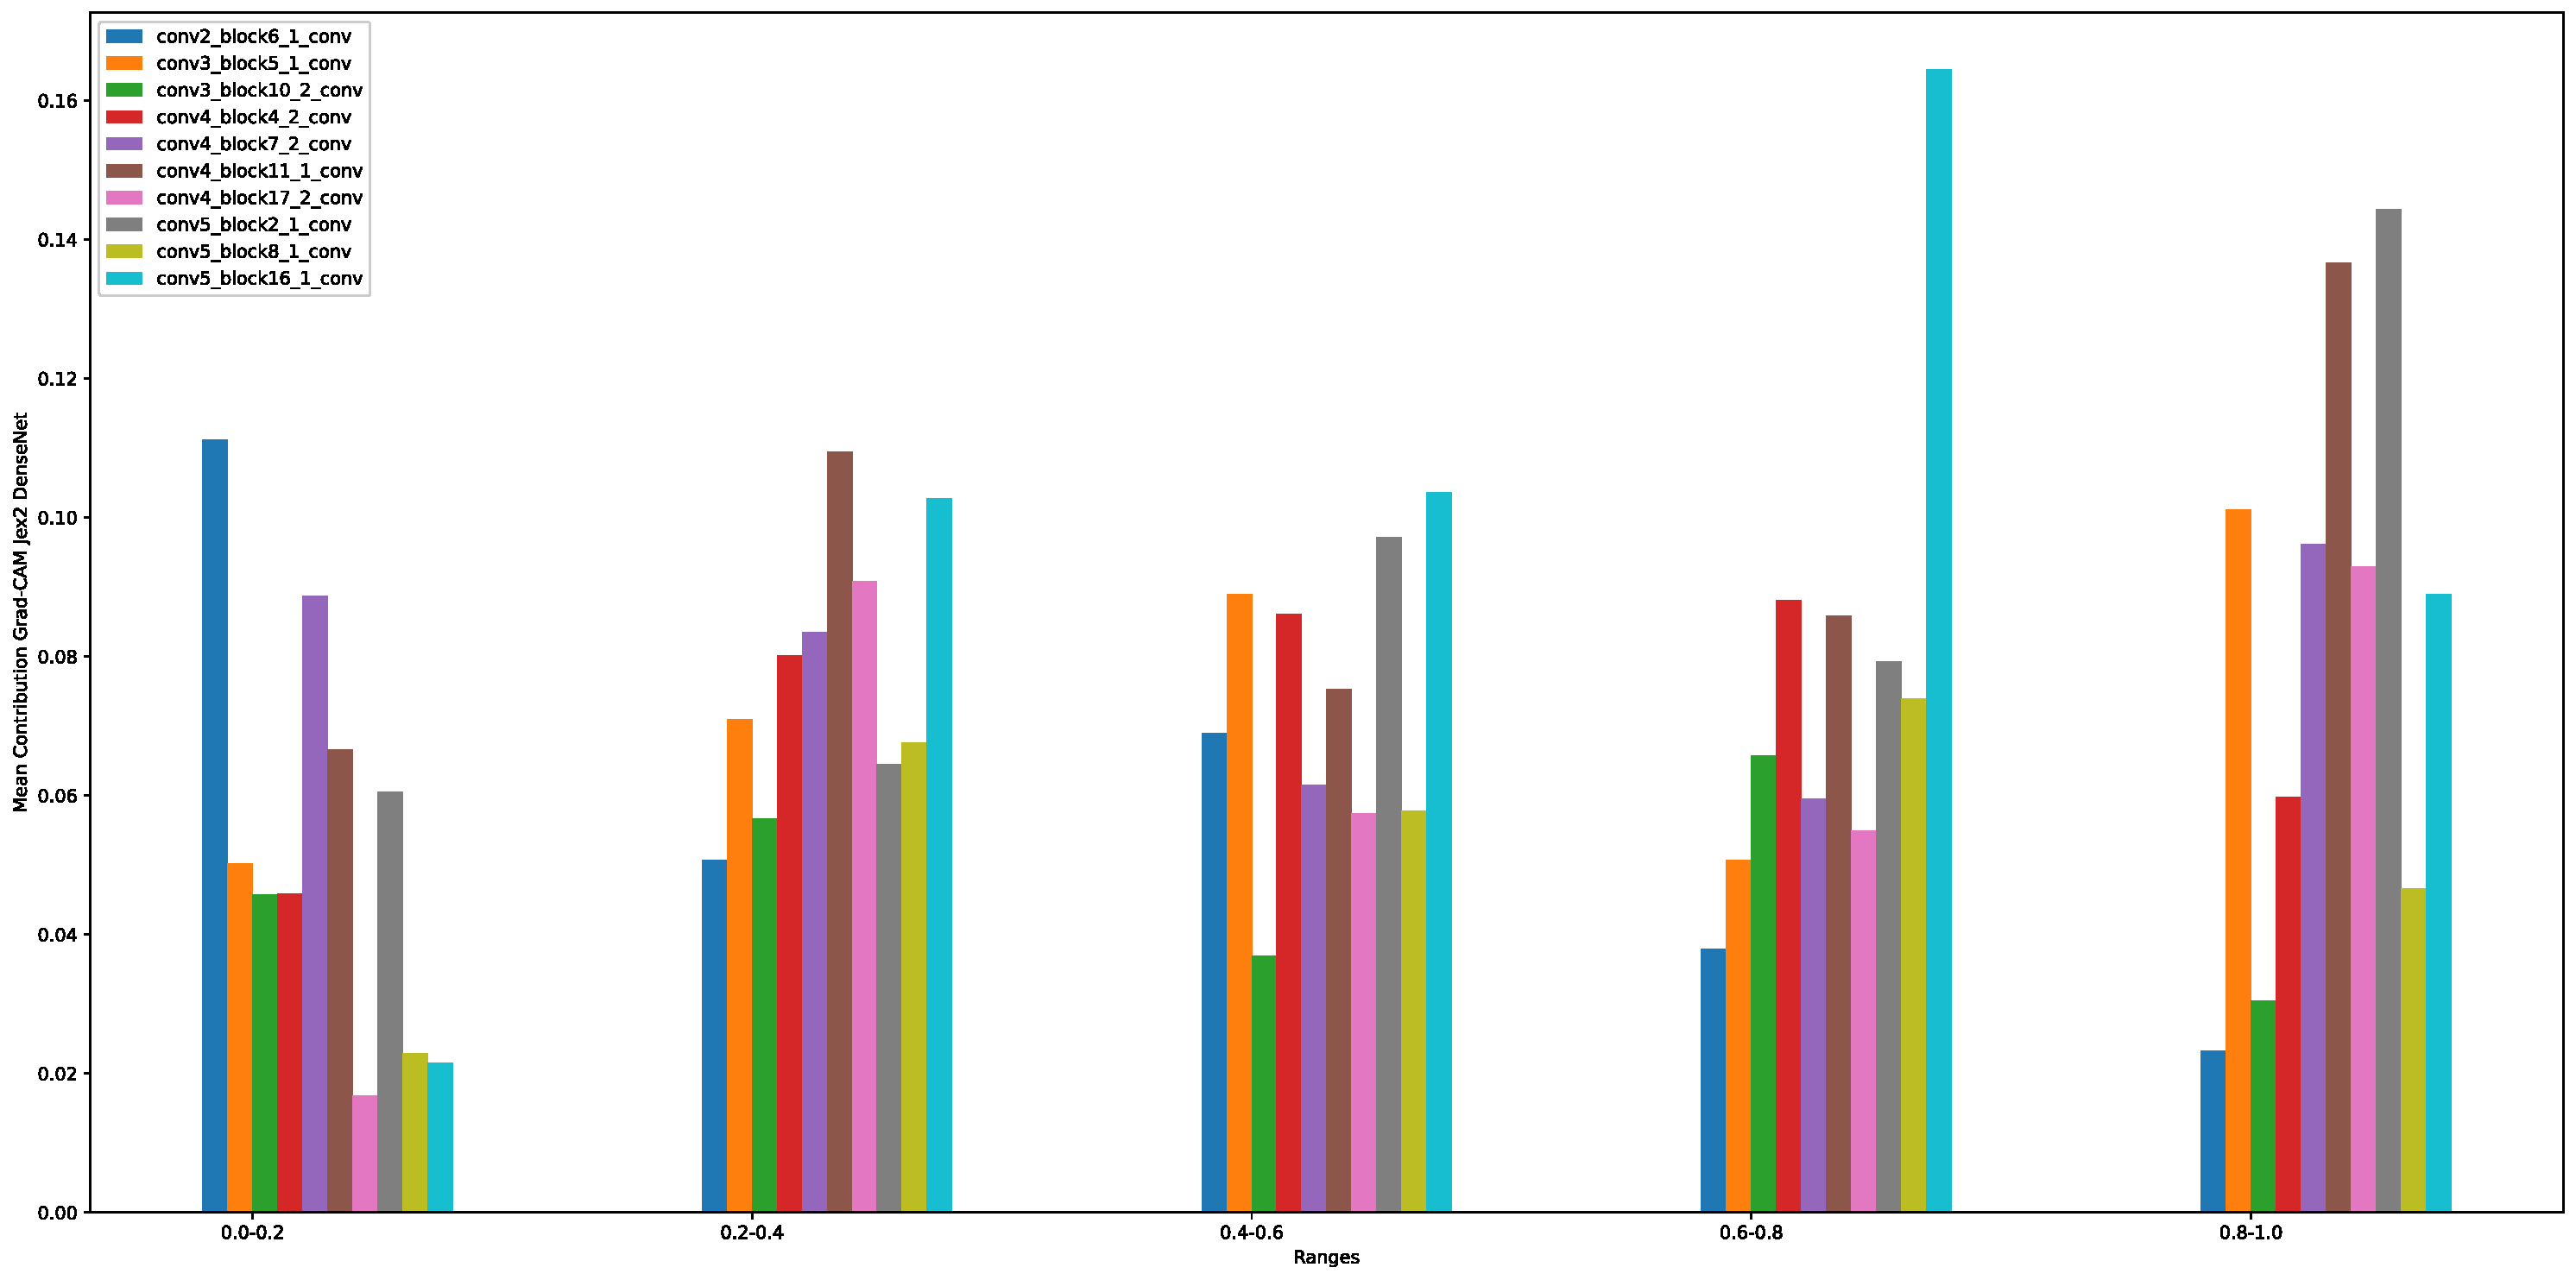
\includegraphics[width=0.85\linewidth]{Figures/mean_contribution_gradcam2.pdf}
    \caption{ Cumulative activation maps per convolutional layer across five predefined KDM value ranges }
    \label{fig:gradcam_cumulative}
\end{figure}
\FloatBarrier



\section{Conclusions}\label{sec:conclusion}

%Párrafo 4: 
%Describa en una sentencia su propuesta (Se desarrolló una metodología de xxx o un método de xx  para xxx a partir de xxx). Recuerde incluir el complemento de la palabra metodología o método o esquema (una metodología de caracterización, clasificación, xx..). Luego enuncie las partes fundamentales y las suposiciones principales de su propuesta, con base a los materiales y métodos declarados. Describa en que bases de datos se validó y bajo qué condiciones, incluyendo medidas de desempeño y propuestas de comparación del estado del arte. Enuncie que dieron los resultados y por qué dichos resultados evidencian la mejora obtenida con su propuesta.


%future work

%En un párrafo aparte enuncie el trabajo futuro por hacer teniendo en cuenta las limitantes tanto teóricas y/o experimentales de su propuesta, y las posibles alternativas de aplicación de su propuesta.



\section*{Acknowledgments}

%% Loading bibliography style file
% \bibliographystyle{model1-num-names}
\bibliographystyle{cas-model2-names}
% \bibliographystyle{ieeetr}

% Loading bibliography database
\bibliography{references}

%Se recomiendan no más de 10 para artículos de eventos y no menos de 30 para revistas.

%Siga el formato de referencias sugerido por el evento o la revista y revise sus partes principales: 

%Se recomienda trabajar con la opción de exportar cita del google scholar:

%https://scholar.google.es/

%Recuerde que se recomienda citar artículos del estado del arte (no más de 3 o 4 años de antigüedad) y no se sesgue a un solo autor.




\end{document}

